% Options for packages loaded elsewhere
% Options for packages loaded elsewhere
\PassOptionsToPackage{unicode}{hyperref}
\PassOptionsToPackage{hyphens}{url}
\PassOptionsToPackage{dvipsnames,svgnames,x11names}{xcolor}
%
\documentclass[
  10t,
]{article}
\usepackage{xcolor}
\usepackage{amsmath,amssymb}
\setcounter{secnumdepth}{-\maxdimen} % remove section numbering
\usepackage{iftex}
\ifPDFTeX
  \usepackage[T1]{fontenc}
  \usepackage[utf8]{inputenc}
  \usepackage{textcomp} % provide euro and other symbols
\else % if luatex or xetex
  \usepackage{unicode-math} % this also loads fontspec
  \defaultfontfeatures{Scale=MatchLowercase}
  \defaultfontfeatures[\rmfamily]{Ligatures=TeX,Scale=1}
\fi
\usepackage{lmodern}
\ifPDFTeX\else
  % xetex/luatex font selection
\fi
% Use upquote if available, for straight quotes in verbatim environments
\IfFileExists{upquote.sty}{\usepackage{upquote}}{}
\IfFileExists{microtype.sty}{% use microtype if available
  \usepackage[]{microtype}
  \UseMicrotypeSet[protrusion]{basicmath} % disable protrusion for tt fonts
}{}
\makeatletter
\@ifundefined{KOMAClassName}{% if non-KOMA class
  \IfFileExists{parskip.sty}{%
    \usepackage{parskip}
  }{% else
    \setlength{\parindent}{0pt}
    \setlength{\parskip}{6pt plus 2pt minus 1pt}}
}{% if KOMA class
  \KOMAoptions{parskip=half}}
\makeatother
% Make \paragraph and \subparagraph free-standing
\makeatletter
\ifx\paragraph\undefined\else
  \let\oldparagraph\paragraph
  \renewcommand{\paragraph}{
    \@ifstar
      \xxxParagraphStar
      \xxxParagraphNoStar
  }
  \newcommand{\xxxParagraphStar}[1]{\oldparagraph*{#1}\mbox{}}
  \newcommand{\xxxParagraphNoStar}[1]{\oldparagraph{#1}\mbox{}}
\fi
\ifx\subparagraph\undefined\else
  \let\oldsubparagraph\subparagraph
  \renewcommand{\subparagraph}{
    \@ifstar
      \xxxSubParagraphStar
      \xxxSubParagraphNoStar
  }
  \newcommand{\xxxSubParagraphStar}[1]{\oldsubparagraph*{#1}\mbox{}}
  \newcommand{\xxxSubParagraphNoStar}[1]{\oldsubparagraph{#1}\mbox{}}
\fi
\makeatother

\usepackage{color}
\usepackage{fancyvrb}
\newcommand{\VerbBar}{|}
\newcommand{\VERB}{\Verb[commandchars=\\\{\}]}
\DefineVerbatimEnvironment{Highlighting}{Verbatim}{commandchars=\\\{\}}
% Add ',fontsize=\small' for more characters per line
\usepackage{framed}
\definecolor{shadecolor}{RGB}{248,248,248}
\newenvironment{Shaded}{\begin{snugshade}}{\end{snugshade}}
\newcommand{\AlertTok}[1]{\textcolor[rgb]{0.94,0.16,0.16}{#1}}
\newcommand{\AnnotationTok}[1]{\textcolor[rgb]{0.56,0.35,0.01}{\textbf{\textit{#1}}}}
\newcommand{\AttributeTok}[1]{\textcolor[rgb]{0.13,0.29,0.53}{#1}}
\newcommand{\BaseNTok}[1]{\textcolor[rgb]{0.00,0.00,0.81}{#1}}
\newcommand{\BuiltInTok}[1]{#1}
\newcommand{\CharTok}[1]{\textcolor[rgb]{0.31,0.60,0.02}{#1}}
\newcommand{\CommentTok}[1]{\textcolor[rgb]{0.56,0.35,0.01}{\textit{#1}}}
\newcommand{\CommentVarTok}[1]{\textcolor[rgb]{0.56,0.35,0.01}{\textbf{\textit{#1}}}}
\newcommand{\ConstantTok}[1]{\textcolor[rgb]{0.56,0.35,0.01}{#1}}
\newcommand{\ControlFlowTok}[1]{\textcolor[rgb]{0.13,0.29,0.53}{\textbf{#1}}}
\newcommand{\DataTypeTok}[1]{\textcolor[rgb]{0.13,0.29,0.53}{#1}}
\newcommand{\DecValTok}[1]{\textcolor[rgb]{0.00,0.00,0.81}{#1}}
\newcommand{\DocumentationTok}[1]{\textcolor[rgb]{0.56,0.35,0.01}{\textbf{\textit{#1}}}}
\newcommand{\ErrorTok}[1]{\textcolor[rgb]{0.64,0.00,0.00}{\textbf{#1}}}
\newcommand{\ExtensionTok}[1]{#1}
\newcommand{\FloatTok}[1]{\textcolor[rgb]{0.00,0.00,0.81}{#1}}
\newcommand{\FunctionTok}[1]{\textcolor[rgb]{0.13,0.29,0.53}{\textbf{#1}}}
\newcommand{\ImportTok}[1]{#1}
\newcommand{\InformationTok}[1]{\textcolor[rgb]{0.56,0.35,0.01}{\textbf{\textit{#1}}}}
\newcommand{\KeywordTok}[1]{\textcolor[rgb]{0.13,0.29,0.53}{\textbf{#1}}}
\newcommand{\NormalTok}[1]{#1}
\newcommand{\OperatorTok}[1]{\textcolor[rgb]{0.81,0.36,0.00}{\textbf{#1}}}
\newcommand{\OtherTok}[1]{\textcolor[rgb]{0.56,0.35,0.01}{#1}}
\newcommand{\PreprocessorTok}[1]{\textcolor[rgb]{0.56,0.35,0.01}{\textit{#1}}}
\newcommand{\RegionMarkerTok}[1]{#1}
\newcommand{\SpecialCharTok}[1]{\textcolor[rgb]{0.81,0.36,0.00}{\textbf{#1}}}
\newcommand{\SpecialStringTok}[1]{\textcolor[rgb]{0.31,0.60,0.02}{#1}}
\newcommand{\StringTok}[1]{\textcolor[rgb]{0.31,0.60,0.02}{#1}}
\newcommand{\VariableTok}[1]{\textcolor[rgb]{0.00,0.00,0.00}{#1}}
\newcommand{\VerbatimStringTok}[1]{\textcolor[rgb]{0.31,0.60,0.02}{#1}}
\newcommand{\WarningTok}[1]{\textcolor[rgb]{0.56,0.35,0.01}{\textbf{\textit{#1}}}}

\usepackage{longtable,booktabs,array}
\usepackage{calc} % for calculating minipage widths
% Correct order of tables after \paragraph or \subparagraph
\usepackage{etoolbox}
\makeatletter
\patchcmd\longtable{\par}{\if@noskipsec\mbox{}\fi\par}{}{}
\makeatother
% Allow footnotes in longtable head/foot
\IfFileExists{footnotehyper.sty}{\usepackage{footnotehyper}}{\usepackage{footnote}}
\makesavenoteenv{longtable}
\usepackage{graphicx}
\makeatletter
\newsavebox\pandoc@box
\newcommand*\pandocbounded[1]{% scales image to fit in text height/width
  \sbox\pandoc@box{#1}%
  \Gscale@div\@tempa{\textheight}{\dimexpr\ht\pandoc@box+\dp\pandoc@box\relax}%
  \Gscale@div\@tempb{\linewidth}{\wd\pandoc@box}%
  \ifdim\@tempb\p@<\@tempa\p@\let\@tempa\@tempb\fi% select the smaller of both
  \ifdim\@tempa\p@<\p@\scalebox{\@tempa}{\usebox\pandoc@box}%
  \else\usebox{\pandoc@box}%
  \fi%
}
% Set default figure placement to htbp
\def\fps@figure{htbp}
\makeatother





\setlength{\emergencystretch}{3em} % prevent overfull lines

\providecommand{\tightlist}{%
  \setlength{\itemsep}{0pt}\setlength{\parskip}{0pt}}



 


% --- Your modified preamble.tex begins here ---
\usepackage[a4paper]{geometry}
\frenchspacing
\tolerance=400
\emergencystretch=3em
\hyphenpenalty=20

\usepackage{unicode-math}
\setmainfont{STIX Two Text}
\setmathfont{STIX Two Math}
\usepackage{mhchem}  % Chemical formula support

% Sans‐serif headings → Fira Sans (with TeX discretionary ligatures)
\setsansfont[
  UprightFont = *-Regular,
  ItalicFont = *-Italic,
  BoldFont = *-Bold,
  BoldItalicFont = *-BoldItalic,
  Ligatures = {TeX, Common, Discretionary},
  Numbers = {Proportional}
]{Fira Sans}

% Monospace Font
\setmonofont[Scale=0.89]{FiraCode Nerd Font}

\usepackage{microtype}
\microtypesetup{
  tracking = true,
  protrusion = true,
  expansion = true,
  factor = 1100,
  stretch = 15,
  shrink = 15,
}

\let\oldtexttt\texttt
\renewcommand{\texttt}[1]{\oldtexttt{\small #1}}
\usepackage{etoolbox}
\AtBeginEnvironment{Highlighting}{\footnotesize}
\AtBeginEnvironment{verbatim}{\footnotesize}
\AtBeginEnvironment{Shaded}{\footnotesize}
\makeatletter
\@ifpackageloaded{caption}{}{\usepackage{caption}}
\AtBeginDocument{%
\ifdefined\contentsname
  \renewcommand*\contentsname{Table of contents}
\else
  \newcommand\contentsname{Table of contents}
\fi
\ifdefined\listfigurename
  \renewcommand*\listfigurename{List of Figures}
\else
  \newcommand\listfigurename{List of Figures}
\fi
\ifdefined\listtablename
  \renewcommand*\listtablename{List of Tables}
\else
  \newcommand\listtablename{List of Tables}
\fi
\ifdefined\figurename
  \renewcommand*\figurename{Figure}
\else
  \newcommand\figurename{Figure}
\fi
\ifdefined\tablename
  \renewcommand*\tablename{Table}
\else
  \newcommand\tablename{Table}
\fi
}
\@ifpackageloaded{float}{}{\usepackage{float}}
\floatstyle{ruled}
\@ifundefined{c@chapter}{\newfloat{codelisting}{h}{lop}}{\newfloat{codelisting}{h}{lop}[chapter]}
\floatname{codelisting}{Listing}
\newcommand*\listoflistings{\listof{codelisting}{List of Listings}}
\makeatother
\makeatletter
\makeatother
\makeatletter
\@ifpackageloaded{caption}{}{\usepackage{caption}}
\@ifpackageloaded{subcaption}{}{\usepackage{subcaption}}
\makeatother
\makeatletter
\@ifpackageloaded{sidenotes}{}{\usepackage{sidenotes}}
\@ifpackageloaded{marginnote}{}{\usepackage{marginnote}}
\makeatother
\usepackage{bookmark}
\IfFileExists{xurl.sty}{\usepackage{xurl}}{} % add URL line breaks if available
\urlstyle{same}
\hypersetup{
  pdftitle={BCB744: Intro R Test},
  pdfauthor={Smit, A. J.},
  colorlinks=true,
  linkcolor={blue},
  filecolor={blue},
  citecolor={blue},
  urlcolor={blue},
  pdfcreator={LaTeX via pandoc}}


\title{BCB744: Intro R Test}
\author{Smit, A. J.}
\date{2025-03-17}
\begin{document}
\maketitle


\section{About the test}\label{about-the-test}

The Intro R Test will start at 8:30 on 17 March, 2025 and you have until
08:30 on 18 March to complete it. The Theory Test must be conducted on
campus, and the Practical Test at home or anywhere you are comfortable
working. The test constitutes a key component of Continuous Assessment
(CA) and are designed to prepare you for the final exam.

The test consists of two parts:

\subsection{Theory Test (30\%)}\label{theory-test-30}

This is a written, closed-book assessment where you will be tested on
theoretical concepts. The only resource available during this test is
RStudio, the R help system, your memory, and your mind.

\subsection{Practical Test (70\%)}\label{practical-test-70}

In this open-book coding assessment, you will apply your theoretical
knowledge to real data problems. While you may reference online
materials (including ChatGPT), collaboration with peers is strictly
prohibited.

\section{Assessment Policy}\label{assessment-policy}

{The marks indicated for each section reflect the relative weight (and
hence depth expected in your response) rather than a rigid checklist of
individual points.} Your answer should demonstrate a comprehensive
understanding of the concepts and techniques required, showing
thoughtful integration of multiple R skills. Higher marks will be
awarded for solutions that demonstrate not only technical correctness
but also elegant code, insightful analysis, and clear communication of
findings. We are assessing your ability to think systematically through
complex data problems, make appropriate methodological choices, and
present your findings in a coherent narrative that reveals meaningful
patterns in the data. Your code should be well-structured, adequately
commented, and reflect good programming practices.

Please refer to the
\href{https://tangledbank.netlify.app/BCB744/BCB744_index.html\#sec-policy}{Assessment
Policy} for more information on the test format and rules.

\section{Theory Test}\label{theory-test}

{\textbf{This is the closed book assessment.}}

Below is a set of questions to answer. You must answer all questions in
the allocated time of 3-hr. Please write your answers in a neatly
formatted Word document and submit it to the iKamva platform.

Clearly indicate the question number and provide detailed explanations
for your answers. Use Word's headings and subheadings facility to
structure your document logically.

Naming convention: \texttt{Intro\_R\_Test\_Theory\_YourSurname.docx}

\subsection{Question 1}\label{question-1}

You are a research assistant who have just been given your first job.
You are asked to analyse a dataset about patterns of extreme heat in the
ocean and the possible role that ocean currents (specifically, eddies)
might play in modulating the patterns of extreme sea surface temperature
extremes in space and time.

Being naive and relatively inexperienced, and misguided by your
exaggerated sense of preparedness as young people tend to do, you gladly
accept the task and start by exploring the data. You notice that the
dataset is quite large, and you have no idea what's happening, what you
are doing, why you are doing it, or what you are looking for. Ten
minutes into the job you start to question your life choices. Your
feeling of bewilderment is compounded by the fact that, when you examine
the data (the output of the \texttt{head()} and \texttt{tail()} commands
is shown below), the entries seem confusing.

\begin{Shaded}
\begin{Highlighting}[]
\NormalTok{fpath }\OtherTok{\textless{}{-}} \StringTok{"/Volumes/OceanData/spatial/processed/WBC/misc\_results"}
\NormalTok{fname }\OtherTok{\textless{}{-}} \StringTok{"KC{-}MCA{-}data{-}2013{-}01{-}01{-}2022{-}12{-}31{-}bbox{-}v1\_ma\_14day\_detrended.csv"}
\NormalTok{data }\OtherTok{\textless{}{-}} \FunctionTok{read.csv}\NormalTok{(}\FunctionTok{file.path}\NormalTok{(fpath, fname))}
\end{Highlighting}
\end{Shaded}

\begin{Shaded}
\begin{Highlighting}[]
\SpecialCharTok{\textgreater{}} \FunctionTok{nrow}\NormalTok{(data)}
\NormalTok{[}\DecValTok{1}\NormalTok{] }\DecValTok{53253434}

\SpecialCharTok{\textgreater{}} \FunctionTok{head}\NormalTok{(data)}
\NormalTok{           t     lon    lat      ex    ke}
\DecValTok{1} \DecValTok{2013{-}01{-}01} \FloatTok{121.875} \FloatTok{34.625} \SpecialCharTok{{-}}\FloatTok{0.7141} \FloatTok{2e{-}04}
\DecValTok{2} \DecValTok{2013{-}01{-}01} \FloatTok{121.875} \FloatTok{34.625} \SpecialCharTok{{-}}\FloatTok{0.8027} \FloatTok{2e{-}04}
\DecValTok{3} \DecValTok{2013{-}01{-}02} \FloatTok{121.875} \FloatTok{34.625} \SpecialCharTok{{-}}\FloatTok{0.8916} \FloatTok{2e{-}04}
\DecValTok{4} \DecValTok{2013{-}01{-}02} \FloatTok{121.875} \FloatTok{34.625} \SpecialCharTok{{-}}\FloatTok{0.9751} \FloatTok{2e{-}04}
\DecValTok{5} \DecValTok{2013{-}01{-}03} \FloatTok{121.875} \FloatTok{34.625} \SpecialCharTok{{-}}\FloatTok{1.0589} \FloatTok{3e{-}04}
\DecValTok{6} \DecValTok{2013{-}01{-}03} \FloatTok{121.875} \FloatTok{34.625} \SpecialCharTok{{-}}\FloatTok{1.1406} \FloatTok{3e{-}04}

\SpecialCharTok{\textgreater{}} \FunctionTok{tail}\NormalTok{(data)}
\NormalTok{                  t     lon    lat     ex      ke}
\DecValTok{53253429} \DecValTok{2022{-}12{-}29} \FloatTok{174.375} \FloatTok{44.875} \FloatTok{0.4742} \SpecialCharTok{{-}}\FloatTok{0.0049}
\DecValTok{53253430} \DecValTok{2022{-}12{-}29} \FloatTok{174.375} \FloatTok{44.875} \FloatTok{0.4856} \SpecialCharTok{{-}}\FloatTok{0.0049}
\DecValTok{53253431} \DecValTok{2022{-}12{-}30} \FloatTok{174.375} \FloatTok{44.875} \FloatTok{0.4969} \SpecialCharTok{{-}}\FloatTok{0.0050}
\DecValTok{53253432} \DecValTok{2022{-}12{-}30} \FloatTok{174.375} \FloatTok{44.875} \FloatTok{0.5169} \SpecialCharTok{{-}}\FloatTok{0.0050}
\DecValTok{53253433} \DecValTok{2022{-}12{-}31} \FloatTok{174.375} \FloatTok{44.875} \FloatTok{0.5367} \SpecialCharTok{{-}}\FloatTok{0.0051}
\DecValTok{53253434} \DecValTok{2022{-}12{-}31} \FloatTok{174.375} \FloatTok{44.875} \FloatTok{0.5465} \SpecialCharTok{{-}}\FloatTok{0.0051}
\end{Highlighting}
\end{Shaded}

You resign yourself to admitting that you don't understand much, but at
the risk of sounding like a fool when you go to your professor, you
decide to do as much of the preparation you can do so that you at least
have something to show for your time.

\begin{enumerate}
\def\labelenumi{\alph{enumi}.}
\tightlist
\item
  What will you take back to your professor to show that you have
  prepared yourself as fully as possible? For example:

  \begin{itemize}
  \tightlist
  \item
    What is in your ability to understand about the study and the nature
    of the data?
  \item
    What will you do for yourself to better understand the task at hand?
  \item
    What do you understand about the data?
  \item
    What will you do to aid your understanding of the data?
  \item
    What will your next steps be going forward?
  \end{itemize}
\item
  What will you need from your professor to help you understand the data
  and the task at hand so that you are well equipped to tackle the
  problem?
\end{enumerate}

\textbf{{[}15 marks{]}}

\textbf{Answer}

\begin{itemize}
\tightlist
\item
  I am able to understand what the concept of `extreme heat' is, and
  what ocean eddies are -- all I need to do is find some papers about it
  and do broad reading around these concepts. So, I will start by
  reading up on these concepts.
\item
  I can see from the columns that there appears to be three independent
  variables (\texttt{lon}, \texttt{lat}, and \texttt{t}) and two
  dependent variables (\texttt{ex} and \texttt{ke}). I will need to
  understand what these variables are, and how they relate to each
  other. It is easy to see that \texttt{lon} and \texttt{lat} are the
  longitude and latitude of the data points, and that \texttt{t} is the
  date of the data point. I will need to understand what the \texttt{ex}
  and \texttt{ke} variables are, and how they relate to the \texttt{lon}
  and \texttt{lat} variables. Presumably \texttt{ex} and \texttt{ke} are
  the extreme heat and ocean eddies, respectively. I'll confirm with the
  professor.
\item
  Because I have \texttt{lon} and \texttt{lat}, I can make a map of the
  study area. By making a map of the study area for one or a few days in
  the dataset, I can get a sense of the spatial distribution of the
  data. I can also plot the \texttt{ex} and \texttt{ke} data to see what
  the data look like. Because the data cover the period 2013-2022, I
  know that I can create a map for each day (a time-series analysis
  might eventually be needed?), and that is probably where the analysis
  will takle me later once I have confirmed my thinking with the
  professor. If I am really proactive and want to seriously impress the
  professor, I'll make an animation of the data to show the temporal
  evolution of revealed patterns in the data over time. This will
  clearly show the processes operating there. A REALLY informed mind
  will be able to even go as far as understanding what the analysis
  shoud entail, but, admittedly, this will require a deep subject matter
  understanding, which you might not possess at the moment, but which is
  nevertheless not beyond your reach to attain without guidance.
\item
  I can conclude that the data reveal some dynamical process (I infer
  `dynamical' from the fact that we have time-series data, and
  time-series reveal dynamics).
\item
  Knowing what the geographical region is from the map I created and
  what is happening there that might be of interest to the study, I can
  make some guesses about what the analysis will be.
\item
  FYI, what basic reseach would reveal include the following (not for
  marks):

  \begin{itemize}
  \tightlist
  \item
    you'd see that it is an ocean region south of South Africa;
  \item
    once you know the region covered, you can read about the processes
    operating in the region that the data cover;
  \item
    because the temperature spatially defines the Agulhas Current, you
    can infer that the study is about the Agulhas Current
  \item
    plotting \texttt{ke} will reveal eddies in the Agulhas Current;
  \item
    you can read about the Agulhas Current and its eddies and think
    about how eddies might affect the temperature in the region -- both
    of these are dynamical processes.
  \end{itemize}
\item
  I will need to understand what the data are telling me, and what the
  variables mean. I will need to understand what the \texttt{ex} and
  \texttt{ke} variables are, and how they relate to the \texttt{lon} and
  \texttt{lat} variables.
\item
  Having discovered all these things simply by doing a basic first-stab
  analyses, I can prepare a report of my cursory findings and draw of a
  list of things I know, toghether with suggested further avenues for
  exploration. I will take this to the professor to confirm my
  understanding and to get guidance on how to proceed.
\item
  I will also add a list of the things I cannot know from the data, and
  what I need to know from the professor to proceed.
\item
  There is also something strange happening with the data. It seems that
  there are duplicate data entries (two occurrences of each combination
  of \texttt{lat} x \texttt{lon} x \texttt{t} resulting in duplicated
  values for each spatio-temporal point of \texttt{ke} and a pair of
  dissimilar values for \texttt{ex}). I will need to understand why this
  is the case. Clearly this is incorrect, and this points to
  pre-processing errors somewhere. I will have to ask the professor to
  give me access to all pro-processing scripts and the raw data to see
  if I can trace the error back to its source.
\item
  If I was this professor, I'd be immensepy mpressed by tyour proactive
  approach to the problem. You are showing that you are not just a
  passive learner, but that you are actively engaging with the data and
  the problem at hand. This is a very good sign of a good researcher in
  the making. In my mind, I'd seriously think about finding you a salary
  for permanent employment in my lab.
\end{itemize}

\subsection{Question 2}\label{question-2}

Please translate the following code into English by providing an
explanation for each line:

\begin{Shaded}
\begin{Highlighting}[]
\NormalTok{monthlyData }\OtherTok{\textless{}{-}}\NormalTok{ dailyData }\SpecialCharTok{\%\textgreater{}\%}
\NormalTok{    dplyr}\SpecialCharTok{::}\FunctionTok{mutate}\NormalTok{(}\AttributeTok{t =} \FunctionTok{asPOSIXct}\NormalTok{(t)) }\SpecialCharTok{\%\textgreater{}\%}
\NormalTok{    dplyr}\SpecialCharTok{::}\FunctionTok{mutate}\NormalTok{(}\AttributeTok{month =} \FunctionTok{floor\_date}\NormalTok{(t, }\AttributeTok{unit =} \StringTok{"month"}\NormalTok{)) }\SpecialCharTok{\%\textgreater{}\%}
\NormalTok{    dplyr}\SpecialCharTok{::}\FunctionTok{group\_by}\NormalTok{(lon, lat, month) }\SpecialCharTok{\%\textgreater{}\%}
\NormalTok{    dplyr}\SpecialCharTok{::}\FunctionTok{summarise}\NormalTok{(}\AttributeTok{temp =} \FunctionTok{mean}\NormalTok{(temp, }\AttributeTok{na.rm =} \ConstantTok{TRUE}\NormalTok{)) }\SpecialCharTok{\%\textgreater{}\%}
\NormalTok{    dplyr}\SpecialCharTok{::}\FunctionTok{mutate}\NormalTok{(}\AttributeTok{year =} \FunctionTok{year}\NormalTok{(month)) }\SpecialCharTok{\%\textgreater{}\%}
\NormalTok{    dplyr}\SpecialCharTok{::}\FunctionTok{group\_by}\NormalTok{(lon, lat) }\SpecialCharTok{\%\textgreater{}\%}
\NormalTok{    dplyr}\SpecialCharTok{::}\FunctionTok{mutate}\NormalTok{(}\AttributeTok{num =} \FunctionTok{seq}\NormalTok{(}\DecValTok{1}\SpecialCharTok{:}\FunctionTok{length}\NormalTok{(temp))) }\SpecialCharTok{\%\textgreater{}\%}
\NormalTok{    dplyr}\SpecialCharTok{::}\FunctionTok{ungroup}\NormalTok{()}
\end{Highlighting}
\end{Shaded}

In your answer, simply refer to the line numbers (1-9) before each line
of code and provide an explanation for each line.

\textbf{{[}10 marks{]}}

\textbf{Answer}

\begin{itemize}
\tightlist
\item
  Line 1: The variable \texttt{monthlyData} is created by starting with
  \texttt{dailyData}, which is a dataset containing daily records.
\item
  Line 2: The \texttt{mutate()} function is used to convert the column
  \texttt{t} (presumably a date or timestamp) into a POSIXct datetime
  format. This ensures that \texttt{t} is stored in a standardised
  date-time format suitable for time-based operations.
\item
  Line 3: The \texttt{mutate()} function is again used to create a new
  column \texttt{month}, which is derived from \texttt{t}. The
  \texttt{floor\_date()} function rounds down the date to the first day
  of the corresponding month, effectively extracting the month from
  \texttt{t}.
\item
  Line 4: The \texttt{group\_by()} function groups the dataset by
  \texttt{lon} (longitude), \texttt{lat} (latitude), and \texttt{month}.
  This means subsequent operations will be performed separately for each
  unique combination of these three variables.
\item
  Line 5: The \texttt{summarise()} function computes the mean
  temperature (\texttt{temp}) for each group. The
  \texttt{na.rm\ =\ TRUE} argument ensures that missing values
  (\texttt{NA}) are ignored in the calculation.
\item
  Line 6: The \texttt{mutate()} function creates a new column,
  \texttt{year}, extracting the year from the \texttt{month} column.
  This provides an explicit reference to the year of each data entry.
\item
  Line 7: The \texttt{group\_by()} function is applied again, but this
  time only by \texttt{lon} and \texttt{lat}. This modifies the grouping
  structure to remove the month grouping while retaining spatial
  grouping.
\item
  Line 8: \texttt{The\ mutate()} function adds a new column,
  \texttt{num}, which assigns a sequence of numbers
  (\texttt{1:length(temp)}) to the grouped data. This effectively
  creates an index for each record within each longitude-latitude group.
\item
  Line 9: The \texttt{ungroup()} function removes all grouping, ensuring
  that further operations on \texttt{monthlyData} are performed on the
  entire dataset rather than within groups.
\end{itemize}

\subsection{Question 3}\label{question-3}

What is `Occam's Razor'?

\textbf{{[}5 marks{]}}

\textbf{Answer}

Occam's Razor is sometimes attributed to the 14th-century philosopher
William of Ockham, is a principle of parsimony that states: ``Entities
should not be multiplied beyond necessity.'' It is relevant to the
BCB744 module because the principle of Occam's Razor is often
interpreted as ``the simplest explanation that sufficiently explains the
data should be preferred over more complex alternatives.'' This is a
nice guiding principle which might be useful in your research,
especially when you are faced with multiple explanations for a
phenomenon. The principle suggests that the simplest explanation is
often the best one, and that more complex explanations should only be
considered when the simpler ones fail to account for the data. But, keep
in mind that biological systems tend to be complex, and oversimplifying
an explanation may ignore important interactions or heterogeneities.

\subsection{Question 4}\label{question-4}

Explain the difference between R and RStudio.

\textbf{{[}5 marks{]}}

\textbf{Answer}

Taken verbatim from Tangled Bank:

\textbf{R is a programming language and software environment for
statistical computing and graphics}. It provides a wide variety of
statistical (linear and non-linear modelling, classical statistical
tests, time-series analysis, classification, clustering, multivariate
analyses, neural networks, and so forth) and graphical techniques, and
is highly extensible.

\textbf{RStudio is an integrated development environment (IDE)} for R.
It provides a graphical user interface (GUI) for working with R, making
it easier to use for those who are less familiar with command-line
interfaces. Some of the features provided by RStudio include:

\begin{itemize}
\tightlist
\item
  a code editor with syntax highlighting and code completion;
\item
  a console for running R code;
\item
  a graphical interface for managing packages and libraries;
\item
  an integrated tools for plotting and visualisation; and
\item
  support for version control with Git and SVN.
\end{itemize}

R is the core software for statistical computing, like a car's engine,
while RStudio provides a more user-friendly interface for working with
R, like the car's body, the seats, steering wheel, and other bells and
whistles.

\subsection{Question 5}\label{question-5}

By way of example, please explain some key aspects of R code
conventions. For each line of code, explain also in English what aspects
of the code are being adhered to.

For example:

\begin{enumerate}
\def\labelenumi{\arabic{enumi}.}
\tightlist
\item
  \texttt{a\ \textless{}-\ b} is not the same as
  \texttt{a\ \textless{}\ -b}. The former is correct because there is a
  space preceding and following the assignment operator
  (\texttt{\textless{}-}, a less-than sign immediately followed by a
  dash to form an arrow); this has a different meaning from the latter,
  which is incorrect because there is no space between the less-than
  sign and the dash, reading as ``a is less than negative b''.
\end{enumerate}

{Hint: In your Word document, use a fixed-width font to indicate the
code as a separate block which is distinct from the rest of the text.}

\textbf{{[}10 marks{]}}

\textbf{Answer}

\begin{enumerate}
\def\labelenumi{\arabic{enumi}.}
\tightlist
\item
  Proper use of indentation:
\end{enumerate}

\begin{Shaded}
\begin{Highlighting}[]
\ControlFlowTok{if}\NormalTok{ (x }\SpecialCharTok{\textgreater{}} \DecValTok{0}\NormalTok{) \{}
  \FunctionTok{print}\NormalTok{(}\StringTok{"Positive number"}\NormalTok{)}
\NormalTok{\}}
\end{Highlighting}
\end{Shaded}

\begin{enumerate}
\def\labelenumi{\arabic{enumi}.}
\setcounter{enumi}{1}
\tightlist
\item
  Use of meaningful variable names:
\end{enumerate}

\begin{Shaded}
\begin{Highlighting}[]
\NormalTok{temperature }\OtherTok{\textless{}{-}} \DecValTok{25}
\end{Highlighting}
\end{Shaded}

\begin{enumerate}
\def\labelenumi{\arabic{enumi}.}
\setcounter{enumi}{2}
\tightlist
\item
  Use of comments to explain code:
\end{enumerate}

\begin{Shaded}
\begin{Highlighting}[]
\CommentTok{\# Calculate the mean temperature}
\NormalTok{mean\_temp }\OtherTok{\textless{}{-}} \FunctionTok{mean}\NormalTok{(temperature)}
\end{Highlighting}
\end{Shaded}

\begin{enumerate}
\def\labelenumi{\arabic{enumi}.}
\setcounter{enumi}{3}
\tightlist
\item
  Consistent use of spacing around operators:
\end{enumerate}

\begin{Shaded}
\begin{Highlighting}[]
\NormalTok{a }\OtherTok{\textless{}{-}}\NormalTok{ b }\SpecialCharTok{+}\NormalTok{ c}
\end{Highlighting}
\end{Shaded}

\begin{enumerate}
\def\labelenumi{\arabic{enumi}.}
\setcounter{enumi}{4}
\tightlist
\item
  Consistent use of compound object names:
\end{enumerate}

A principles of writing clean and readable R code (or \emph{any} code)
is maintaining consistent variable naming conventions throughout a
script or project. Mixing different naming styles -- such as
``snake\_case'' (words separated by underscores) and ``camelCase''
(capitalising the first letter of each subsequent word) -- makes the
code harder to read, maintain, and debug.

Examples:

\begin{Shaded}
\begin{Highlighting}[]
\CommentTok{\# Example of consistent use of either convention:}
\NormalTok{my\_variable }\OtherTok{\textless{}{-}} \DecValTok{10} \CommentTok{\# snake case}
\NormalTok{another\_variable }\OtherTok{\textless{}{-}} \DecValTok{20} \CommentTok{\# camel case}

\CommentTok{\# An example of inconsistent use of conventions:}
\NormalTok{myVariable }\OtherTok{\textless{}{-}} \DecValTok{30} \CommentTok{\# camel case}
\NormalTok{yet\_another\_variable }\OtherTok{\textless{}{-}} \DecValTok{40} \CommentTok{\# snake case}

\CommentTok{\# This is also incorrect:}
\NormalTok{variable\_one }\OtherTok{\textless{}{-}} \DecValTok{13} \CommentTok{\# llowercase "one"}
\NormalTok{variable\_Two }\OtherTok{\textless{}{-}} \DecValTok{13} \SpecialCharTok{*} \DecValTok{2} \CommentTok{\# uppercase "Two"}
\end{Highlighting}
\end{Shaded}

\begin{enumerate}
\def\labelenumi{\arabic{enumi}.}
\setcounter{enumi}{5}
\tightlist
\item
  Avoiding the = as Assignment Operator
\end{enumerate}

\begin{Shaded}
\begin{Highlighting}[]
\CommentTok{\# Correct:}
\NormalTok{a }\OtherTok{\textless{}{-}} \DecValTok{1}

\CommentTok{\# Incorrect:}
\NormalTok{a }\OtherTok{=} \DecValTok{1}
\end{Highlighting}
\end{Shaded}

\begin{enumerate}
\def\labelenumi{\arabic{enumi}.}
\setcounter{enumi}{6}
\tightlist
\item
  Consistent use of spaces around \# symbols in comments:
\end{enumerate}

\begin{Shaded}
\begin{Highlighting}[]
\CommentTok{\# This is correct:}

\CommentTok{\# This is a comment}
\CommentTok{\# This is another comment}
\CommentTok{\# And another}

\CommentTok{\# This is incorrect:}

\CommentTok{\#This is a comment}
\CommentTok{\# A comment?}
\CommentTok{\#  Another comment}
\end{Highlighting}
\end{Shaded}

\begin{enumerate}
\def\labelenumi{\arabic{enumi}.}
\setcounter{enumi}{7}
\tightlist
\item
  Correct use of \texttt{+} or \texttt{-} for unary operators:
\end{enumerate}

\begin{Shaded}
\begin{Highlighting}[]
\CommentTok{\# Correct:}
\NormalTok{a }\OtherTok{\textless{}{-}} \SpecialCharTok{{-}}\NormalTok{b}
\end{Highlighting}
\end{Shaded}

\begin{enumerate}
\def\labelenumi{\arabic{enumi}.}
\setcounter{enumi}{8}
\tightlist
\item
  Use of \texttt{TRUE} and \texttt{FALSE} instead of \texttt{T} and
  \texttt{F}:
\end{enumerate}

\begin{Shaded}
\begin{Highlighting}[]
\CommentTok{\# Correct:}
\NormalTok{is\_positive }\OtherTok{\textless{}{-}} \ConstantTok{TRUE}

\CommentTok{\# Incorrect:}
\NormalTok{is\_positive }\OtherTok{\textless{}{-}}\NormalTok{ T}
\end{Highlighting}
\end{Shaded}

For more, refer to the
\href{https://style.tidyverse.org/syntax.html}{tidyverse style guide}.

\subsection{Question 6}\label{question-6}

\begin{enumerate}
\def\labelenumi{\alph{enumi}.}
\tightlist
\item
  Explain why one typically prefers working with CSV files over Excel
  files in R.
\item
  What are the properties of a CSV file that make it more suitable for
  data analysis in R?
\item
  What are the properties of an Excel file that make it less suitable
  for data analysis in R?
\end{enumerate}

\textbf{{[}15 marks{]}}

\textbf{Answer}

\begin{enumerate}
\def\labelenumi{\alph{enumi})}
\tightlist
\item
\end{enumerate}

CSV (Comma-Separated Values) files are preferred over Excel files due to
their simplicity, compatibility, and efficiency in handling data. CSV
files are stored as plain text, making them easy to read and write
across different software and platforms. They do not contain proprietary
formatting, formulas, or metadata, which minimises the risk of
unintended data transformations.

Excel files (.xls, .xlsx) are proprietary and designed for spreadsheet
applications, incorporating complex formatting, formulas, and visual
formatting that can interfere with data processing in R. Unlike CSV
files, which can be directly read using base R functions like
\texttt{read.csv()}, Excel files require additional packages such as
\textbf{readxl} for data extraction. Excel's tendency to automatically
modify data types -- such as converting text to dates or numbers -- is
annoying and introduces errors, making CSV a more reliable format for
reproducible data analysis.

\begin{enumerate}
\def\labelenumi{\alph{enumi})}
\setcounter{enumi}{1}
\tightlist
\item
\end{enumerate}

\begin{itemize}
\tightlist
\item
  CSV files store data in a simple text-based format that ensures easy
  readability by both humans and computers.
\item
  Each row represents a single record, and fields are separated by
  commas (or another delimiter) to ensure a consistent tabular format.
\item
  CSV files can be opened and edited using a wide range of software,
  including text editors, spreadsheets (e.g., Excel, Google Sheets), and
  statistical tools (e.g., R, Python).
\item
  R provides optimised functions like \texttt{read.csv()} (base R) and
  \texttt{read\_csv()} (tidyverse) for quickly reading CSV files without
  additional dependencies.
\item
  Unlike Excel, CSV files do not contain embedded formulas, formatting,
  figures, or macros and these properties reduce the risk of unintended
  data stuff-ups.
\item
  Being plain text, CSV files are typically smaller in size compared to
  Excel files.
\end{itemize}

\begin{enumerate}
\def\labelenumi{\alph{enumi})}
\setcounter{enumi}{2}
\tightlist
\item
\end{enumerate}

\begin{itemize}
\tightlist
\item
  Excel files are stored in a format (.xls, .xlsx) that is specific to
  Microsoft Excel; special packages (e.g., \textbf{readxl},
  \textbf{openxlsx}) are needed to read them in R.
\item
  Excel often automatically formats data and changes numeric values to
  dates or rounding decimal values. This can lead to errors in data
  analysis.
\item
  Excel files support formulas, pivot tables, conditional formatting,
  and visual elements that may not be relevant for raw data processing
  in R.
\item
  Users can store multiple sheets within a single Excel file and this
  makes it trickier to maintain a standardised structure when importing
  data into R.
\item
  Excel files are not made for handling large datasets. Excel becomes
  very slow and is prone to crashing or memory limitations when dealing
  with `big' data.
\item
  Excel's binary files do not work with version control systems like
  Git.
\item
  Excel files are complex and more prone to accidental modifications or
  corruption.
\end{itemize}

\subsection{Question 7}\label{question-7}

Explain each of the following in the context of their use in R. For
each, provide an example of how you would construct them in R:

\begin{enumerate}
\def\labelenumi{\alph{enumi}.}
\tightlist
\item
  A vector
\item
  A matrix
\item
  A dataframe
\item
  A list
\end{enumerate}

Hint: See my hint under Question 5.

\textbf{{[}20 marks{]}}

\textbf{Answer}

\begin{enumerate}
\def\labelenumi{(\alph{enumi})}
\tightlist
\item
  A vector in R is the simplest and most fundamental data structure. It
  is a one-dimensional collection of elements, all of the same type
  (e.g., numeric, character, or logical). Vectors can be created using
  the \texttt{c()} function. For example:
\end{enumerate}

\begin{Shaded}
\begin{Highlighting}[]
\CommentTok{\# Creating a numeric vector}
\NormalTok{numbers }\OtherTok{\textless{}{-}} \FunctionTok{c}\NormalTok{(}\DecValTok{1}\NormalTok{, }\DecValTok{2}\NormalTok{, }\DecValTok{3}\NormalTok{, }\DecValTok{4}\NormalTok{, }\DecValTok{5}\NormalTok{)}

\CommentTok{\# Creating a character vector}
\NormalTok{names }\OtherTok{\textless{}{-}} \FunctionTok{c}\NormalTok{(}\StringTok{"Acacia"}\NormalTok{, }\StringTok{"Protea"}\NormalTok{, }\StringTok{"Leucadendron"}\NormalTok{)}

\CommentTok{\# Creating a logical vector}
\NormalTok{logical\_values }\OtherTok{\textless{}{-}} \FunctionTok{c}\NormalTok{(}\ConstantTok{TRUE}\NormalTok{, }\ConstantTok{FALSE}\NormalTok{, }\ConstantTok{TRUE}\NormalTok{)}
\end{Highlighting}
\end{Shaded}

\begin{enumerate}
\def\labelenumi{(\alph{enumi})}
\setcounter{enumi}{1}
\tightlist
\item
  A matrix is a two-dimensional data structure where all elements must
  be of the same type. It is essentially an extension of a vector with a
  specified number of rows and columns.
\end{enumerate}

\begin{Shaded}
\begin{Highlighting}[]
\CommentTok{\# Creating a matrix with 3 rows and 2 columns}
\NormalTok{my\_matrix }\OtherTok{\textless{}{-}} \FunctionTok{matrix}\NormalTok{(}\FunctionTok{c}\NormalTok{(}\DecValTok{1}\NormalTok{, }\DecValTok{2}\NormalTok{, }\DecValTok{3}\NormalTok{, }\DecValTok{4}\NormalTok{, }\DecValTok{5}\NormalTok{, }\DecValTok{6}\NormalTok{), }\AttributeTok{nrow =} \DecValTok{3}\NormalTok{, }\AttributeTok{ncol =} \DecValTok{2}\NormalTok{)}
\end{Highlighting}
\end{Shaded}

\begin{enumerate}
\def\labelenumi{(\alph{enumi})}
\setcounter{enumi}{2}
\tightlist
\item
  A dataframe is a two-dimensional data structure that can contain
  different data types in different columns (variables). It is the most
  commonly used data structure for data analysis in R and resembles a
  table with rows and columns.
\end{enumerate}

\begin{Shaded}
\begin{Highlighting}[]
\CommentTok{\# Creating a dataframe}
\NormalTok{my\_dataframe }\OtherTok{\textless{}{-}} \FunctionTok{data.frame}\NormalTok{(}
  \AttributeTok{Name =} \FunctionTok{c}\NormalTok{(}\StringTok{"Acacia"}\NormalTok{, }\StringTok{"Protea"}\NormalTok{, }\StringTok{"Leucadendron"}\NormalTok{),}
  \AttributeTok{Age =} \FunctionTok{c}\NormalTok{(}\DecValTok{25}\NormalTok{, }\DecValTok{30}\NormalTok{, }\DecValTok{22}\NormalTok{),}
  \AttributeTok{Height =} \FunctionTok{c}\NormalTok{(}\FloatTok{85.5}\NormalTok{, }\FloatTok{90.3}\NormalTok{, }\FloatTok{78.0}\NormalTok{)}
\NormalTok{)}
\end{Highlighting}
\end{Shaded}

\begin{enumerate}
\def\labelenumi{(\alph{enumi})}
\setcounter{enumi}{3}
\tightlist
\item
  A list is a flexible data structure that can store elements of
  different types, including vectors, matrices, dataframes, and even
  other lists. Unlike vectors and matrices, which require uniform data
  types, lists can contain heterogeneous elements.
\end{enumerate}

\begin{Shaded}
\begin{Highlighting}[]
\CommentTok{\# Creating a list with different data types}
\CommentTok{\# Uses the data created abobe, for example}
\NormalTok{my\_list }\OtherTok{\textless{}{-}} \FunctionTok{list}\NormalTok{(}
  \AttributeTok{plants =}\NormalTok{ my\_dataframe,}
  \AttributeTok{some\_numbers =}\NormalTok{ mu\_matrix,}
  \AttributeTok{other\_numbers =}\NormalTok{ numbers}
\NormalTok{  )}
\end{Highlighting}
\end{Shaded}

\subsection{Question 8}\label{question-8}

\begin{enumerate}
\def\labelenumi{\alph{enumi}.}
\item
  Write a 150 to 200 word abstract about your Honours research project.
  In your abstract, draw attention to the types of data you will be
  expected to generate, and mention how these will be used to address
  your research question.
\item
  Explain which of the R data classes will be most useful in your
  research and why.
\item
  With reference to the abstract you wrote in Question 8.a, explain how
  you would visualise (or display your finding in tabular format) your
  research findings. Provide an example of how you would do this in R.
  Which of your research questions would be best answered using a
  visualisations or tables? What do you expect your visualisations or
  tables to show?
\item
  Provide an example of how you would create a plot or table in R.
  Generate mock code (it does not need to run) that you would use to
  create the plot or table.
\end{enumerate}

Note 1: In the unlikely event that your research will not require
visualisations or tables, please explain why this is the case and how
you would communicate your findings.

Note 2: If you haven't defined your research project yet, describe a
hypothetical project in your field of interest.

\textbf{{[}30 marks{]}}

\textbf{Answer}

This will have to be assessed based on the information quality produced
in each abstract. Assign marks as follows:

\begin{enumerate}
\def\labelenumi{\alph{enumi}.}
\tightlist
\item
  Abstract: 30\%
\item
  Data classes: 10\%
\item
  Visualisation: 30\%
\item
  Mock code: 30\%
\end{enumerate}

\textbf{TOTAL MARKS: 110}

\section{Practical Test}\label{practical-test}

{\textbf{This is the open book assessment.}}

Below is a set of scripting problems to solve. You have 21 hours from
the end of the Theory Test to complete this section Please write your
code in an R script file and submit it to the iKamva platform by no
later than 8:30 on Tuesday, 18 March 2025.

Please follow a clear structure (appropriate, clearly numbered headings
and subheadings) in your code, including comments and explanations.

{Ensure that all code runs without errors before submitting it --
serious penalties will apply to non-functional scripts.}

Naming convention: \texttt{Intro\_R\_Test\_Practical\_YourSurname.R}

\subsection{Question 1}\label{question-1-1}

Download the
\href{https://raw.githubusercontent.com/ajsmit/R_courses/main/static/data/fertiliser_crop_data.csv}{\texttt{fertiliser\_crop\_data.csv}}
data.

The data represent an experiment designed to test whether or not
fertiliser type and the density of planting have an effect on the yield
of wheat. The dataset contains the following variables:

\begin{itemize}
\tightlist
\item
  Final yield (kg per acre) -- make sure to convert this to the most
  suitable SI unit before continuing with your analysis
\item
  Type of fertiliser (fertiliser type A, B, or C)
\item
  Planting density (1 = low density, 2 = high density)
\item
  Block in the field (north, east, south, west)
\end{itemize}

Undertake a full visual assessment of the dataset and establish which of
the influential variables are most likely to have an effect on crop
yield. Provide a detailed explanation of your findings.

\textbf{{[}25 marks{]}}

\textbf{Answer}

First, ensure the data are converted to SI units (e.g., kg per hectare)
for consistency. I'd examine the tops and bottoms of the data with
\texttt{head()} and \texttt{tail()} to see what we are dealing with, and
it's also useful to do a \texttt{summary()}. I'd also print a table to
see how the various measurements are distributed across the predictor
variables.

\begin{Shaded}
\begin{Highlighting}[]
\FunctionTok{library}\NormalTok{(tidyverse)}
\FunctionTok{library}\NormalTok{(ggpubr)}
\NormalTok{fert }\OtherTok{\textless{}{-}} \FunctionTok{read.csv}\NormalTok{(}\StringTok{"../data/fertiliser\_crop\_data.csv"}\NormalTok{)}

\CommentTok{\# Convert to SI units}
\NormalTok{fert }\OtherTok{\textless{}{-}}\NormalTok{ fert }\SpecialCharTok{|\textgreater{}}
  \FunctionTok{mutate}\NormalTok{(}\AttributeTok{mass =}\NormalTok{ mass }\SpecialCharTok{/} \FloatTok{0.40468564224}\NormalTok{)}

\CommentTok{\# Convert acre to ha}
\NormalTok{fert }\OtherTok{\textless{}{-}}\NormalTok{ fert }\SpecialCharTok{|\textgreater{}}
  \FunctionTok{mutate}\NormalTok{(}\AttributeTok{mass =}\NormalTok{ mass }\SpecialCharTok{*} \FloatTok{2.47105}\NormalTok{)}

\CommentTok{\# Check the data}
\FunctionTok{head}\NormalTok{(fert)}
\end{Highlighting}
\end{Shaded}

\begin{verbatim}
  density block fertilizer     mass
1       1 north          A 29451.95
2       2  east          A 29505.35
3       1 south          A 29315.65
4       2  west          A 29530.88
5       1 north          A 29434.80
6       2  east          A 29377.11
\end{verbatim}

\begin{Shaded}
\begin{Highlighting}[]
\FunctionTok{tail}\NormalTok{(fert)}
\end{Highlighting}
\end{Shaded}

\begin{verbatim}
   density block fertilizer     mass
91       1 south          C 29445.18
92       2  west          C 29481.30
93       1 north          C 29603.67
94       2  east          C 29532.04
95       1 south          C 29528.16
96       2  west          C 29433.59
\end{verbatim}

\begin{Shaded}
\begin{Highlighting}[]
\FunctionTok{summary}\NormalTok{(fert)}
\end{Highlighting}
\end{Shaded}

\begin{verbatim}
    density       block            fertilizer             mass      
 Min.   :1.0   Length:96          Length:96          Min.   :29142  
 1st Qu.:1.0   Class :character   Class :character   1st Qu.:29326  
 Median :1.5   Mode  :character   Mode  :character   Median :29424  
 Mean   :1.5                                         Mean   :29417  
 3rd Qu.:2.0                                         3rd Qu.:29480  
 Max.   :2.0                                         Max.   :29756  
\end{verbatim}

\begin{Shaded}
\begin{Highlighting}[]
\CommentTok{\# Create a table showing the grouping structure of block, density, and fertiliser}
\NormalTok{fert }\SpecialCharTok{\%\textgreater{}\%}
  \FunctionTok{group\_by}\NormalTok{(block, density, fertilizer) }\SpecialCharTok{|\textgreater{}} 
  \FunctionTok{summarise}\NormalTok{(}\AttributeTok{n =} \FunctionTok{n}\NormalTok{()) }\SpecialCharTok{|\textgreater{}} 
  \FunctionTok{head}\NormalTok{(}\DecValTok{12}\NormalTok{)}
\end{Highlighting}
\end{Shaded}

\begin{verbatim}
# A tibble: 12 x 4
# Groups:   block, density [4]
   block density fertilizer     n
   <chr>   <int> <chr>      <int>
 1 east        2 A              8
 2 east        2 B              8
 3 east        2 C              8
 4 north       1 A              8
 5 north       1 B              8
 6 north       1 C              8
 7 south       1 A              8
 8 south       1 B              8
 9 south       1 C              8
10 west        2 A              8
11 west        2 B              8
12 west        2 C              8
\end{verbatim}

Then, I'd calculate the mean and standard deviation of the outcome
variable for each level of the independent variables. This will give me
a sense of the central tendency and spread of the data.

\begin{Shaded}
\begin{Highlighting}[]
\CommentTok{\# Let\textquotesingle{}s see group differences}
\CommentTok{\# I also calculate the mean +/{-} SD here}
\NormalTok{fert }\SpecialCharTok{|\textgreater{}} 
  \FunctionTok{group\_by}\NormalTok{(density) }\SpecialCharTok{|\textgreater{}} 
  \FunctionTok{summarise}\NormalTok{(}\AttributeTok{mean =} \FunctionTok{mean}\NormalTok{(mass),}
            \AttributeTok{SD =} \FunctionTok{sd}\NormalTok{(mass))}
\end{Highlighting}
\end{Shaded}

\begin{verbatim}
# A tibble: 2 x 3
  density   mean    SD
    <int>  <dbl> <dbl>
1       1 29378.  101.
2       2 29455.  107.
\end{verbatim}

\begin{Shaded}
\begin{Highlighting}[]
\NormalTok{fert }\SpecialCharTok{|\textgreater{}} 
  \FunctionTok{group\_by}\NormalTok{(block) }\SpecialCharTok{|\textgreater{}} 
  \FunctionTok{summarise}\NormalTok{(}\AttributeTok{mean =} \FunctionTok{mean}\NormalTok{(mass),}
            \AttributeTok{SD =} \FunctionTok{sd}\NormalTok{(mass))}
\end{Highlighting}
\end{Shaded}

\begin{verbatim}
# A tibble: 4 x 3
  block   mean    SD
  <chr>  <dbl> <dbl>
1 east  29467. 107. 
2 north 29390. 104. 
3 south 29366.  98.2
4 west  29443. 108. 
\end{verbatim}

\begin{Shaded}
\begin{Highlighting}[]
\NormalTok{fert }\SpecialCharTok{|\textgreater{}} 
  \FunctionTok{group\_by}\NormalTok{(fertilizer) }\SpecialCharTok{|\textgreater{}} 
  \FunctionTok{summarise}\NormalTok{(}\AttributeTok{mean =} \FunctionTok{mean}\NormalTok{(mass),}
            \AttributeTok{SD =} \FunctionTok{sd}\NormalTok{(mass))}
\end{Highlighting}
\end{Shaded}

\begin{verbatim}
# A tibble: 3 x 3
  fertilizer   mean    SD
  <chr>       <dbl> <dbl>
1 A          29374. 114. 
2 B          29403.  95.4
3 C          29473.  99.6
\end{verbatim}

Next, I'd create plots of the data showing each level of independent
variables that the outcome can vary over. Boxplots and barplots are the
most appropriate, together with some form of variance indication (SE,
SD, or CI).

\begin{Shaded}
\begin{Highlighting}[]
\CommentTok{\# Visual assessment}
\CommentTok{\# Create a boxplot of mass by density, fertiliser type, and density}
\CommentTok{\# ... by fertiliser}
\NormalTok{plt1 }\OtherTok{\textless{}{-}}\NormalTok{ fert }\SpecialCharTok{|\textgreater{}} 
  \FunctionTok{ggplot}\NormalTok{(}\FunctionTok{aes}\NormalTok{(}\AttributeTok{x =}\NormalTok{ block, }\AttributeTok{y =}\NormalTok{ mass, }\AttributeTok{fill =} \FunctionTok{as.factor}\NormalTok{(density))) }\SpecialCharTok{+}
  \FunctionTok{geom\_boxplot}\NormalTok{(}\AttributeTok{notch =} \ConstantTok{FALSE}\NormalTok{) }\SpecialCharTok{+}
  \FunctionTok{labs}\NormalTok{(}\AttributeTok{x =} \StringTok{"Fertiliser type"}\NormalTok{,}
       \AttributeTok{y =} \StringTok{"Crop yield (kg/ha)"}\NormalTok{,}
       \AttributeTok{fill =} \StringTok{"Planting}\SpecialCharTok{\textbackslash{}n}\StringTok{density"}\NormalTok{)}

\CommentTok{\# ... by density()}
\NormalTok{plt2 }\OtherTok{\textless{}{-}}\NormalTok{ fert }\SpecialCharTok{|\textgreater{}} 
  \FunctionTok{ggplot}\NormalTok{(}\FunctionTok{aes}\NormalTok{(}\AttributeTok{x =}\NormalTok{ block, }\AttributeTok{y =}\NormalTok{ mass, }\AttributeTok{fill =}\NormalTok{ fertilizer)) }\SpecialCharTok{+}
  \FunctionTok{geom\_boxplot}\NormalTok{(}\AttributeTok{notch =} \ConstantTok{FALSE}\NormalTok{) }\SpecialCharTok{+}
  \FunctionTok{labs}\NormalTok{(}\AttributeTok{x =} \StringTok{"Block"}\NormalTok{,}
       \AttributeTok{y =} \StringTok{"Crop yield (kg/ha)"}\NormalTok{,}
       \AttributeTok{fill =} \StringTok{"Fertiliser}\SpecialCharTok{\textbackslash{}n}\StringTok{type"}\NormalTok{)}

\NormalTok{plt3 }\OtherTok{\textless{}{-}}\NormalTok{ fert }\SpecialCharTok{|\textgreater{}} 
  \FunctionTok{ggplot}\NormalTok{(}\FunctionTok{aes}\NormalTok{(}\AttributeTok{x =} \FunctionTok{as.factor}\NormalTok{(density), }\AttributeTok{y =}\NormalTok{ mass, }\AttributeTok{fill =}\NormalTok{ fertilizer)) }\SpecialCharTok{+}
  \FunctionTok{geom\_boxplot}\NormalTok{(}\AttributeTok{notch =} \ConstantTok{FALSE}\NormalTok{) }\SpecialCharTok{+}
  \FunctionTok{labs}\NormalTok{(}\AttributeTok{x =} \StringTok{"Planting density"}\NormalTok{,}
       \AttributeTok{y =} \StringTok{"Crop yield (kg/ha)"}\NormalTok{,}
       \AttributeTok{fill =} \StringTok{"Fertiliser}\SpecialCharTok{\textbackslash{}n}\StringTok{type"}\NormalTok{)}

\CommentTok{\# Arrange the plots}
\FunctionTok{ggarrange}\NormalTok{(plt1, plt2, plt3, }\AttributeTok{ncol =} \DecValTok{2}\NormalTok{, }\AttributeTok{nrow =} \DecValTok{2}\NormalTok{, }\AttributeTok{labels =} \StringTok{"AUTO"}\NormalTok{)}
\end{Highlighting}
\end{Shaded}

\pandocbounded{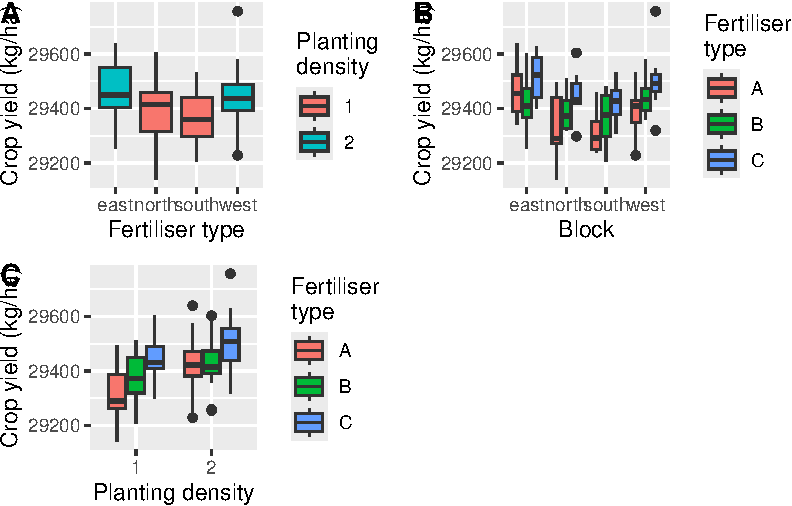
\includegraphics[keepaspectratio]{BCB744_Intro_R_Test_2025_files/figure-pdf/unnamed-chunk-19-1.pdf}}

I'd then interpret these results, considering on the inferences I can
make from visual assessments of the mean (or median) and the figures.
The analyses must take into account all the influential variables:
density, block, and fertiliser. Since this is Intro R and not
Biostatistics, inferential stats tests aren't expected.

\begin{itemize}
\tightlist
\item
  I'd note that the mass of crop produced by fertiliser C is the
  greatest compared to both A and B; the effect of fertiliser B is no
  different (at least not consistently) than that of A. This response is
  seen if viewed across the different blocks and densities.
\item
  The second planting density also yields a greater mass per ha, but it
  is also confounded with the block, so I'd need to consider this in my
  interpretation\ldots{} East and west blocks have the highest yield,
  but they also were planted at a higher density to start with. To
  circumvent this problem, maybe calculate something like a yield per
  plant, a yield per unit area, or even relative growth rate, and then
  compare these across the different blocks and densities.
\item
  These interpretations can be reached from examining the boxplots (or
  barplots) and the median (or mean), and some measure of variance such
  as ±SD (or ±CI).
\end{itemize}

For some bonus marks, I'd also consider the limitations of the study and
potential confounding variables that may have influenced the results.

\begin{itemize}
\tightlist
\item
  I mentioned the confounding of block with density, but I'd also
  consider other factors that could have influenced the results, such as
  soil quality, weather conditions, or other unmeasured variables. None
  of these are mentioned, so the student can draw attention to this as
  unknowns that could affect the outcome.
\end{itemize}

\subsection{Question 2}\label{question-2-1}

The Bullfrog Occupancy and Common Reed Invasion data are here:
\texttt{AICcmodavg::bullfrog} (i.e.~the \texttt{bullfrogs} dataset
resides within the \textbf{AICcmodavg} package, which you might have to
install).

Create a tidy dataframe from the bullfrog data.

\textbf{{[}10 marks{]}}

\textbf{Answer}

\begin{Shaded}
\begin{Highlighting}[]
\FunctionTok{library}\NormalTok{(AICcmodavg)}
\FunctionTok{data}\NormalTok{(bullfrog)}

\CommentTok{\# View the first/last few rows of the dataset}
\FunctionTok{head}\NormalTok{(bullfrog)}
\end{Highlighting}
\end{Shaded}

\begin{verbatim}
                       Location Reed.presence V1 V2 V3 V4 V5 V6 V7    Effort1
1                  Arbo_Mc_gill             0  0  0  0  0  0  0  0  1.3342857
2            Beauharnois_bassin             1  0  0  0  0  0  0  0 -0.6657143
3            Beauharnois_chemin             1  0  0  0  0  0  0  0 -0.6657143
4           Bois_de_liesse_elec             1  0 NA NA  0 NA NA  0 -4.6657143
5          Bois_de_liesse_grand             0  0  0  0  0  0  0  0  2.3342857
6 IBoucherville_chenal_a_pinard             1  0  0  0  1  0  0  0  0.3342857
     Effort2    Effort3    Effort4    Effort5    Effort6    Effort7 Type1 Type2
1  1.3342857  1.3342857  1.3342857  0.3342857  0.3342857  1.3342857     0     1
2 -0.6657143 -0.6657143 -0.6657143 -0.6657143 -0.6657143 -0.6657143     0     1
3 -0.6657143 -0.6657143 -0.6657143 -0.6657143 -0.6657143 -0.6657143     0     1
4 -8.6657143 -8.6657143 -4.6657143 -8.6657143 -8.6657143 -4.6657143     0     1
5  2.3342857  2.3342857  2.3342857  2.3342857  2.3342857  2.3342857     0     1
6  0.3342857  0.3342857  0.3342857  0.3342857  0.3342857  0.3342857     0     1
  Type3 Type4 Type5 Type6 Type7
1     1     0     1     1     0
2     1     0     1     1     0
3     1     0     1     1     0
4     1     0     1     1     0
5     1     0     1     1     0
6     1     0     1     1     0
\end{verbatim}

\begin{Shaded}
\begin{Highlighting}[]
\CommentTok{\# Convert the data to a tidy dataframe}
\CommentTok{\# place all of the variables \textasciigrave{}V1\textasciigrave{} through \textasciigrave{}V7\textasciigrave{} under a single column}
\CommentTok{\# that represents the survey occasion}
\CommentTok{\# place all the variables \textasciigrave{}Effort1\textasciigrave{} through \textasciigrave{}Effort7\textasciigrave{} under a single}
\CommentTok{\# column that represents the sampling effort}
\CommentTok{\# place all the variables \textasciigrave{}Type1\textasciigrave{} through \textasciigrave{}Type7\textasciigrave{} under a single}
\CommentTok{\# column that represents the survey type}

\CommentTok{\# Reshape the data}
\NormalTok{tidy\_bullfrog }\OtherTok{\textless{}{-}}\NormalTok{ bullfrog }\SpecialCharTok{|\textgreater{}} 
  \FunctionTok{pivot\_longer}\NormalTok{(}\AttributeTok{cols =} \FunctionTok{starts\_with}\NormalTok{(}\StringTok{"V"}\NormalTok{),}
               \AttributeTok{names\_to =} \StringTok{"Occasion"}\NormalTok{,}
               \AttributeTok{values\_to =} \StringTok{"Occasion.val"}\NormalTok{) }\SpecialCharTok{|\textgreater{}} 
  \FunctionTok{pivot\_longer}\NormalTok{(}\AttributeTok{cols =} \FunctionTok{starts\_with}\NormalTok{(}\StringTok{"Effort"}\NormalTok{),}
               \AttributeTok{names\_to =} \StringTok{"Effort"}\NormalTok{,}
               \AttributeTok{values\_to =} \StringTok{"Effort.val"}\NormalTok{) }\SpecialCharTok{|\textgreater{}} 
  \FunctionTok{pivot\_longer}\NormalTok{(}\AttributeTok{cols =} \FunctionTok{starts\_with}\NormalTok{(}\StringTok{"Type"}\NormalTok{),}
               \AttributeTok{names\_to =} \StringTok{"Type"}\NormalTok{,}
               \AttributeTok{values\_to =} \StringTok{"Type.val"}\NormalTok{)}

\CommentTok{\# View the first/last few rows of the tidy dataframe}
\FunctionTok{head}\NormalTok{(tidy\_bullfrog)}
\end{Highlighting}
\end{Shaded}

\begin{verbatim}
# A tibble: 6 x 8
  Location  Reed.presence Occasion Occasion.val Effort Effort.val Type  Type.val
  <fct>             <int> <chr>           <int> <chr>       <dbl> <chr>    <int>
1 Arbo_Mc_~             0 V1                  0 Effor~       1.33 Type1        0
2 Arbo_Mc_~             0 V1                  0 Effor~       1.33 Type2        1
3 Arbo_Mc_~             0 V1                  0 Effor~       1.33 Type3        1
4 Arbo_Mc_~             0 V1                  0 Effor~       1.33 Type4        0
5 Arbo_Mc_~             0 V1                  0 Effor~       1.33 Type5        1
6 Arbo_Mc_~             0 V1                  0 Effor~       1.33 Type6        1
\end{verbatim}

To consider in marking the answer:

\begin{itemize}
\tightlist
\item
  The student should have reshaped the data into a tidy format, with
  each row representing a unique observation.
\item
  The student should have correctly identified the variables to be
  reshaped and the new column names.
\item
  The student should have demonstrated an understanding of the
  \texttt{pivot\_longer()} (or equivalent) function and its arguments.
\item
  They should have applied an consistent naming convention for the new
  columns.
\end{itemize}

\subsection{Question 3}\label{question-3-1}

The Growth Curves for Sitka Spruce Trees in 1988 and 1989 data are here:
\texttt{MASS::Sitka} and \texttt{MASS::Sitka89}.

Combine the two datasets and provide an analysis of the growth curves
for Sitka spruce trees in 1988 and 1989. Give graphical support for the
idea that i) ozone affects the growth of Sitka spruce trees, and ii) the
growth of Sitka spruce trees is affected by the year of measurement. In
addition to showing the overall response in each year x treatment, also
ensure that the among tree variability is visible.

Explain your findings.

\textbf{{[}20 marks{]}}

\textbf{Answer}

\begin{Shaded}
\begin{Highlighting}[]
\CommentTok{\# load data}
\NormalTok{sitka }\OtherTok{\textless{}{-}}\NormalTok{ MASS}\SpecialCharTok{::}\NormalTok{Sitka}
\NormalTok{sitka89 }\OtherTok{\textless{}{-}}\NormalTok{ MASS}\SpecialCharTok{::}\NormalTok{Sitka89}

\CommentTok{\# Look at them}
\FunctionTok{head}\NormalTok{(sitka)}
\end{Highlighting}
\end{Shaded}

\begin{verbatim}
  size Time tree treat
1 4.51  152    1 ozone
2 4.98  174    1 ozone
3 5.41  201    1 ozone
4 5.90  227    1 ozone
5 6.15  258    1 ozone
6 4.24  152    2 ozone
\end{verbatim}

\begin{Shaded}
\begin{Highlighting}[]
\FunctionTok{head}\NormalTok{(sitka89)}
\end{Highlighting}
\end{Shaded}

\begin{verbatim}
  size Time tree treat
1 6.16  469    1 ozone
2 6.18  496    1 ozone
3 6.48  528    1 ozone
4 6.65  556    1 ozone
5 6.87  579    1 ozone
6 6.95  613    1 ozone
\end{verbatim}

\begin{Shaded}
\begin{Highlighting}[]
\CommentTok{\# Combine the two datasets}
\CommentTok{\# rbind them, and create a new column for the year (1988 for \textasciigrave{}Sitka\textasciigrave{} and}
\CommentTok{\# 1989 for \textasciigrave{}Sitka89\textasciigrave{})}
\NormalTok{sitka}\SpecialCharTok{$}\NormalTok{year }\OtherTok{\textless{}{-}} \DecValTok{1988}
\NormalTok{sitka89}\SpecialCharTok{$}\NormalTok{year }\OtherTok{\textless{}{-}} \DecValTok{1989}

\CommentTok{\# Combine the datasets}
\NormalTok{sitka\_combined }\OtherTok{\textless{}{-}} \FunctionTok{rbind}\NormalTok{(sitka, sitka89)}

\CommentTok{\# Make some plots}
\FunctionTok{ggplot}\NormalTok{(}\AttributeTok{data =}\NormalTok{ sitka\_combined, }\FunctionTok{aes}\NormalTok{(}\AttributeTok{x =}\NormalTok{ Time, }\AttributeTok{y =}\NormalTok{ size)) }\SpecialCharTok{+}
  \FunctionTok{geom\_smooth}\NormalTok{(}\FunctionTok{aes}\NormalTok{(}\AttributeTok{group =}\NormalTok{ tree),}
              \AttributeTok{color =} \StringTok{"pink"}\NormalTok{,  }\CommentTok{\# among{-}tree variability lines}
              \AttributeTok{linewidth =} \FloatTok{0.2}\NormalTok{,}
              \AttributeTok{se =} \ConstantTok{FALSE}\NormalTok{) }\SpecialCharTok{+}
  \FunctionTok{geom\_smooth}\NormalTok{(}\FunctionTok{aes}\NormalTok{(}\AttributeTok{color =}\NormalTok{ treat),  }\CommentTok{\# overall lines mapped to treatment}
              \AttributeTok{linewidth =} \DecValTok{1}\NormalTok{,}
              \AttributeTok{se =} \ConstantTok{TRUE}\NormalTok{) }\SpecialCharTok{+}
  \FunctionTok{scale\_color\_manual}\NormalTok{(}\AttributeTok{values =} \FunctionTok{c}\NormalTok{(}\StringTok{"control"} \OtherTok{=} \StringTok{"white"}\NormalTok{, }\StringTok{"ozone"} \OtherTok{=} \StringTok{"black"}\NormalTok{)) }\SpecialCharTok{+}
  \FunctionTok{labs}\NormalTok{(}\AttributeTok{x =} \StringTok{"Time (Days)"}\NormalTok{,}
       \AttributeTok{y =} \StringTok{"Size (m)"}\NormalTok{,}
       \AttributeTok{title =} \StringTok{"Size change over time in 1988 and 1989"}\NormalTok{) }\SpecialCharTok{+}
  \FunctionTok{facet\_wrap}\NormalTok{(}\SpecialCharTok{\textasciitilde{}}\NormalTok{ year, }\AttributeTok{scales =} \StringTok{"free\_x"}\NormalTok{)}
\end{Highlighting}
\end{Shaded}

\pandocbounded{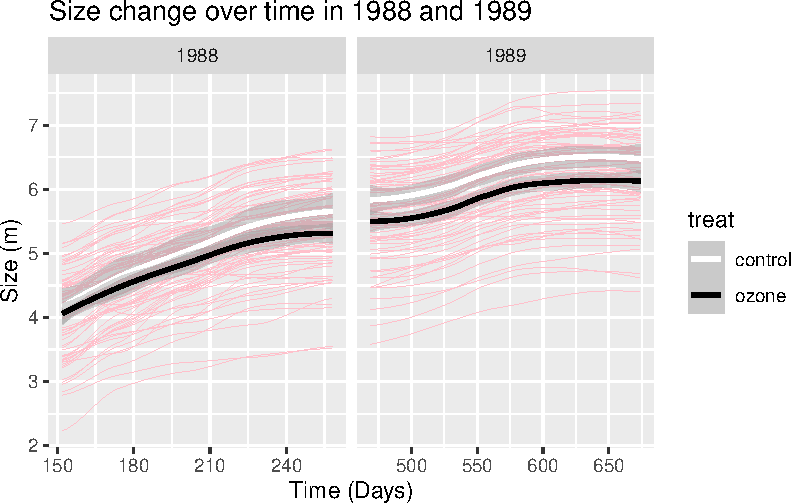
\includegraphics[keepaspectratio]{BCB744_Intro_R_Test_2025_files/figure-pdf/unnamed-chunk-22-1.pdf}}

The figure shows the growth curves for Sitka spruce trees in 1988 and
1989. The pink lines represent the growth curves for individual trees,
while the red and blie lines represent the average growth curves for the
control and ozone-treated trees, respectively. The growth curves for the
ozone-treated trees appear to be lower than those for the control trees,
indicating that ozone affects the growth of Sitka spruce trees.
Additionally, although the trees are all taller in 1989, the growth
curves for 1989 are generally lower (i.e.~their rate of change over
time) than those for 1988, suggesting that the growth of Sitka spruce
trees is affected by the year of measurement. This suggests the trees
are maturing and their growth rates are slowing down. The variability
among trees is also visible and very substantial, with some trees being
bigger in 1988 compared to some in 1989.

\subsection{Question 4}\label{question-4-1}

The Frog Dehydration Experiment on Three Substrate Types data can be
accessed here: \texttt{AICcmodavg::dry.frog}.

\begin{enumerate}
\def\labelenumi{\alph{enumi}.}
\tightlist
\item
  Based on the dataset, what do you think was the purpose of this study?
  Provide a 200 word synopsis as your answer.
\item
  Create new columns in the dataframe showing:

  \begin{itemize}
  \tightlist
  \item
    the final mass;
  \item
    the percent mass lost; and
  \item
    the percent mass lost as a function of the initial mass of each
    frog.
  \end{itemize}
\item
  Provide the R code that would have resulted in the data in the
  variables \texttt{cent\_Initial\_mass} and \texttt{cent\_Air}.
\item
  An analysis of the factors responsible for dehydration rates in frogs.
  In your analysis, consider the effects substrate type, initial mass,
  air temperature, and wind.
\item
  Provide a brief discussion of your findings.
\end{enumerate}

\textbf{{[}25 marks{]}}

\textbf{Answer}

\begin{enumerate}
\def\labelenumi{\alph{enumi}.}
\item
  The investigators sought to determine whether anthropogenic
  disturbances that remove ground cover or alter substrate moisture
  impede the dispersal and homing capacities of frog populations. They
  hypothesised that desiccation risks, heightened predation exposure,
  and substrate temperature extremes could collectively inhibit anuran
  relocations across open landscapes. By scrutinising individual
  orientation behaviour and homing success, they hoped to elucidate
  whether frogs could detect distant patches of suitable habitat and
  whether traversing hostile terrain diminished the likelihood of
  reaching them. They also questioned if contrasting body sizes,
  reflecting differing surface-to-volume ratios, influenced dehydration
  and survival patterns during overland migrations. Seeking mechanistic
  clarity rather than mere distributional data, they devised a series of
  field-based translocation tests, effectively isolating frogs on
  disturbed or undisturbed surfaces to compare path selection, movement
  propensity, and ultimate reunion with their original ponds.
  Additionally, by examining dehydration rates and postural adaptations
  on varied substrates -- ranging from vegetation-rich bogs to dry peat
  fields -- they aimed to quantify physiological constraints that shape
  dispersal outcomes. Through these interconnected experiments, they
  intended to shed further light on the dynamic interplay between
  environmental structure, amphibian behaviour, and survival to inform
  predictive models of habitat connectivity and population resilience in
  areas undergoing increasingly disruptive land-use transformations.
\item
  To calculate the final mass, percent mass lost, and percent mass lost
  as a function of the initial mass of each frog, we can use the
  following code:
\end{enumerate}

\begin{Shaded}
\begin{Highlighting}[]
\FunctionTok{library}\NormalTok{(AICcmodavg)}
\FunctionTok{data}\NormalTok{(dry.frog)}

\CommentTok{\# Looking the data}
\FunctionTok{head}\NormalTok{(dry.frog)}
\end{Highlighting}
\end{Shaded}

\begin{verbatim}
  Individual Species Shade  SVL Substrate Initial_mass Mass_lost Airtemp
1          1   Racla     0 7.27      SOIL         38.5       8.3      31
2          2   Racla     0 7.00  SPHAGNUM         31.0       3.6      31
3          3   Racla     0 6.83      PEAT         23.6       4.7      31
4          4   Racla     0 7.26      PEAT         37.4       7.0      22
5          5   Racla     0 7.43      SOIL         44.4       7.7      22
6          6   Racla     0 5.75  SPHAGNUM         16.4       1.6      22
  Wind_cat Cloud cent_Initial_mass Initial_mass2 cent_Air Perc.cloud Wind
1        3    20         20.361157    414.576715  2.64876       0.20    1
2        3    20         12.861157    165.409360  2.64876       0.20    1
3        3    20          5.461157     29.824236  2.64876       0.20    1
4        2     5         19.261157    370.992170 -6.35124       0.05    1
5        2     5         26.261157    689.648368 -6.35124       0.05    1
6        2     5         -1.738843      3.023575 -6.35124       0.05    1
  log_Mass_lost
1      3.217231
2      2.201634
3      2.510962
4      3.000000
5      3.121015
6      1.378512
\end{verbatim}

\begin{Shaded}
\begin{Highlighting}[]
\CommentTok{\# Create new columns}
\NormalTok{frog }\OtherTok{\textless{}{-}}\NormalTok{ dry.frog }\SpecialCharTok{|\textgreater{}}
  \FunctionTok{mutate}\NormalTok{(}\AttributeTok{Final\_mass =}\NormalTok{ (Initial\_mass }\SpecialCharTok{{-}}\NormalTok{ Mass\_lost)) }\SpecialCharTok{|\textgreater{}}
  \FunctionTok{mutate}\NormalTok{(}\AttributeTok{Perc\_mass\_loss =}\NormalTok{ (Initial\_mass }\SpecialCharTok{/}\NormalTok{ Final\_mass) }\SpecialCharTok{*} \DecValTok{100}\NormalTok{) }\SpecialCharTok{|\textgreater{}} 
  \FunctionTok{mutate}\NormalTok{(}\AttributeTok{Perc\_mass\_loss\_initial =}\NormalTok{ Perc\_mass\_loss) }
\end{Highlighting}
\end{Shaded}

\begin{enumerate}
\def\labelenumi{\alph{enumi}.}
\setcounter{enumi}{2}
\tightlist
\item
  Here, `centered' means to subtract the overall mean from each value.
  The R code that would have resulted in the data in the variables
  \texttt{cent\_Initial\_mass} and \texttt{cent\_Air} is as follows:
\end{enumerate}

\begin{Shaded}
\begin{Highlighting}[]
\CommentTok{\# Create the cent\_Initial\_mass and cent\_Air columns}
\NormalTok{frog }\OtherTok{\textless{}{-}}\NormalTok{ frog }\SpecialCharTok{|\textgreater{}}
  \FunctionTok{mutate}\NormalTok{(}\AttributeTok{cent\_Initial\_mass\_new =}\NormalTok{ (Initial\_mass }\SpecialCharTok{{-}} \FunctionTok{mean}\NormalTok{(Initial\_mass))) }\SpecialCharTok{|\textgreater{}}
  \FunctionTok{mutate}\NormalTok{(}\AttributeTok{cent\_Air\_new =}\NormalTok{ (Airtemp }\SpecialCharTok{{-}} \FunctionTok{mean}\NormalTok{(Airtemp)))}
\end{Highlighting}
\end{Shaded}

\begin{enumerate}
\def\labelenumi{\alph{enumi}.}
\setcounter{enumi}{3}
\tightlist
\item
  To create a purely visual analysis of the factors responsible for
  dehydration rates in frogs, we can trend lines, scatter plots,
  boxplots, etc. examine the effects of substrate type, initial mass,
  air temperature, and wind on the percent mass lost. The code would
  look something like this:
\end{enumerate}

\begin{Shaded}
\begin{Highlighting}[]
\CommentTok{\# Create graphs of all the influential variables and their effects}
\CommentTok{\# on the mass loss:}
\CommentTok{\# ... the effect of substrate}
\NormalTok{plt1 }\OtherTok{\textless{}{-}}\NormalTok{ frog }\SpecialCharTok{|\textgreater{}} 
  \FunctionTok{ggplot}\NormalTok{(}\FunctionTok{aes}\NormalTok{(}\AttributeTok{x =}\NormalTok{ Substrate, }\AttributeTok{y =}\NormalTok{ Perc\_mass\_loss)) }\SpecialCharTok{+}
  \FunctionTok{geom\_boxplot}\NormalTok{() }\SpecialCharTok{+}
  \FunctionTok{labs}\NormalTok{(}\AttributeTok{x =} \StringTok{"Substrate type"}\NormalTok{,}
       \AttributeTok{y =} \StringTok{"Percent mass lost"}\NormalTok{)}

\CommentTok{\# ... the effect of initial mass}
\NormalTok{plt2 }\OtherTok{\textless{}{-}}\NormalTok{ frog }\SpecialCharTok{|\textgreater{}} 
  \FunctionTok{ggplot}\NormalTok{(}\FunctionTok{aes}\NormalTok{(}\AttributeTok{x =}\NormalTok{ Initial\_mass, }\AttributeTok{y =}\NormalTok{ Perc\_mass\_loss)) }\SpecialCharTok{+}
  \FunctionTok{geom\_point}\NormalTok{() }\SpecialCharTok{+}
  \FunctionTok{geom\_smooth}\NormalTok{(}\AttributeTok{method =} \StringTok{"lm"}\NormalTok{) }\SpecialCharTok{+}
  \FunctionTok{labs}\NormalTok{(}\AttributeTok{x =} \StringTok{"Initial mass"}\NormalTok{,}
       \AttributeTok{y =} \StringTok{"Percent mass lost"}\NormalTok{)}

\CommentTok{\# ... the effect of air temperature}
\NormalTok{plt3 }\OtherTok{\textless{}{-}}\NormalTok{ frog }\SpecialCharTok{|\textgreater{}} 
  \FunctionTok{ggplot}\NormalTok{(}\FunctionTok{aes}\NormalTok{(}\AttributeTok{x =}\NormalTok{ Airtemp, }\AttributeTok{y =}\NormalTok{ Perc\_mass\_loss)) }\SpecialCharTok{+}
  \FunctionTok{geom\_point}\NormalTok{() }\SpecialCharTok{+}
  \FunctionTok{geom\_smooth}\NormalTok{(}\AttributeTok{method =} \StringTok{"lm"}\NormalTok{) }\SpecialCharTok{+}
  \FunctionTok{labs}\NormalTok{(}\AttributeTok{x =} \StringTok{"Air temperature"}\NormalTok{,}
       \AttributeTok{y =} \StringTok{"Percent mass lost"}\NormalTok{)}

\CommentTok{\# ... the effect of the wind category}
\NormalTok{plt4 }\OtherTok{\textless{}{-}}\NormalTok{ frog }\SpecialCharTok{|\textgreater{}} 
  \FunctionTok{ggplot}\NormalTok{(}\FunctionTok{aes}\NormalTok{(}\AttributeTok{x =} \FunctionTok{as.factor}\NormalTok{(Wind\_cat), }\AttributeTok{y =}\NormalTok{ Perc\_mass\_loss)) }\SpecialCharTok{+}
  \FunctionTok{geom\_boxplot}\NormalTok{() }\SpecialCharTok{+}
  \FunctionTok{labs}\NormalTok{(}\AttributeTok{x =} \StringTok{"Wind category"}\NormalTok{,}
       \AttributeTok{y =} \StringTok{"Percent mass lost"}\NormalTok{)}

\FunctionTok{ggarrange}\NormalTok{(plt1, plt2, plt3, plt4, }\AttributeTok{ncol =} \DecValTok{2}\NormalTok{, }\AttributeTok{nrow =} \DecValTok{2}\NormalTok{, }\AttributeTok{labels =} \StringTok{"AUTO"}\NormalTok{)}
\end{Highlighting}
\end{Shaded}

\pandocbounded{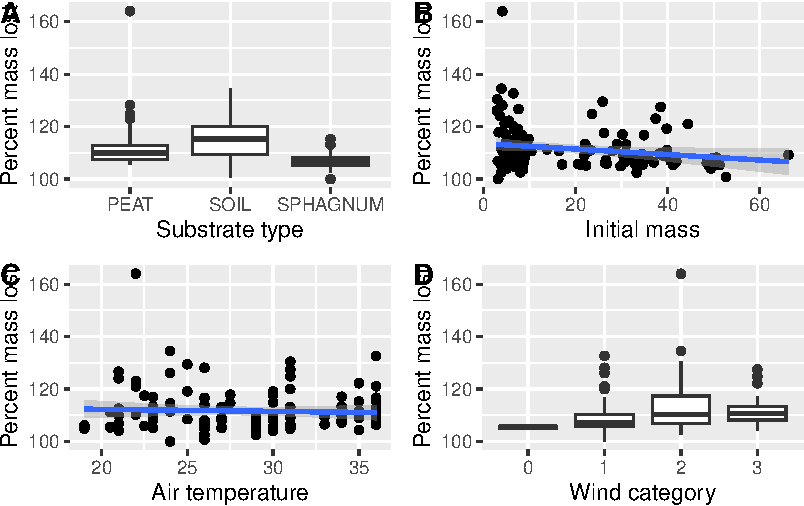
\includegraphics[keepaspectratio]{BCB744_Intro_R_Test_2025_files/figure-pdf/unnamed-chunk-25-1.pdf}}

\begin{enumerate}
\def\labelenumi{\alph{enumi}.}
\setcounter{enumi}{4}
\tightlist
\item
  Frogs on soil showed the largest overall percent‐mass losses, while
  sphagnum moss minimised losses. Larger individuals tended to lose a
  lower fraction of their mass than smaller ones. Temperature had a weak
  negative (or no effect, statistically) trend, whereas stronger wind
  categories tended to correspond to elevated mass‐loss percentages.
\end{enumerate}

\subsection{Question 5}\label{question-5-1}

Consider this script:

\begin{Shaded}
\begin{Highlighting}[]
\FunctionTok{ggplot}\NormalTok{(points, }\FunctionTok{aes}\NormalTok{(}\AttributeTok{x =}\NormalTok{ group, }\AttributeTok{y =}\NormalTok{ count)) }\SpecialCharTok{+}
  \FunctionTok{geom\_boxplot}\NormalTok{(}\FunctionTok{aes}\NormalTok{(}\AttributeTok{colour =}\NormalTok{ group), }\AttributeTok{size =} \DecValTok{1}\NormalTok{, }\AttributeTok{outlier.colour =} \ConstantTok{NA}\NormalTok{) }\SpecialCharTok{+}
  \FunctionTok{geom\_point}\NormalTok{(}\AttributeTok{position =} \FunctionTok{position\_jitter}\NormalTok{(}\AttributeTok{width =} \FloatTok{0.2}\NormalTok{), }\AttributeTok{alpha =} \FloatTok{0.3}\NormalTok{) }\SpecialCharTok{+}
  \FunctionTok{facet\_grid}\NormalTok{(group }\SpecialCharTok{\textasciitilde{}}\NormalTok{ ., }\AttributeTok{scales =} \StringTok{"free"}\NormalTok{) }\SpecialCharTok{+}
  \FunctionTok{labs}\NormalTok{(}\AttributeTok{x =} \StringTok{""}\NormalTok{, }\AttributeTok{y =} \StringTok{"Number of data points"}\NormalTok{) }\SpecialCharTok{+}
  \FunctionTok{theme}\NormalTok{(}\AttributeTok{legend.position =} \StringTok{"none"}\NormalTok{,}
    \AttributeTok{strip.background =} \FunctionTok{element\_blank}\NormalTok{(),}
    \AttributeTok{strip.text =} \FunctionTok{element\_blank}\NormalTok{())}
\end{Highlighting}
\end{Shaded}

\begin{enumerate}
\def\labelenumi{\alph{enumi}.}
\tightlist
\item
  Generate fictitious (random, normal) data that can be plotted using
  the code, above. Make sure to assemble these data into a dataframe
  suitable for plotting, complete with correct column titles.
\item
  Apply the script \emph{exactly as stated} to the data to demonstate
  your understanding of the code and convince the examiner of your
  understanding of the correct data structure.
\end{enumerate}

\textbf{{[}10 marks{]}}

\textbf{Answer}

\begin{enumerate}
\def\labelenumi{\alph{enumi}.}
\tightlist
\item
  Generate the data:
\end{enumerate}

\begin{Shaded}
\begin{Highlighting}[]
\CommentTok{\# Generate some fictitious data}
\FunctionTok{set.seed}\NormalTok{(}\DecValTok{123}\NormalTok{)  }\CommentTok{\# For reproducibility}

\NormalTok{points }\OtherTok{\textless{}{-}} \FunctionTok{data.frame}\NormalTok{(}
  \AttributeTok{group =} \FunctionTok{rep}\NormalTok{(}\FunctionTok{c}\NormalTok{(}\StringTok{"A"}\NormalTok{, }\StringTok{"B"}\NormalTok{, }\StringTok{"C"}\NormalTok{), }\AttributeTok{each =} \DecValTok{30}\NormalTok{),}
  \AttributeTok{count =} \FunctionTok{c}\NormalTok{(}
    \FunctionTok{rnorm}\NormalTok{(}\DecValTok{30}\NormalTok{, }\AttributeTok{mean =} \DecValTok{10}\NormalTok{, }\AttributeTok{sd =} \DecValTok{3}\NormalTok{),}
    \FunctionTok{rnorm}\NormalTok{(}\DecValTok{30}\NormalTok{, }\AttributeTok{mean =} \DecValTok{20}\NormalTok{, }\AttributeTok{sd =} \DecValTok{4}\NormalTok{),}
    \FunctionTok{rnorm}\NormalTok{(}\DecValTok{30}\NormalTok{, }\AttributeTok{mean =} \DecValTok{15}\NormalTok{, }\AttributeTok{sd =} \DecValTok{2}\NormalTok{)}
\NormalTok{  )}
\NormalTok{)}

\CommentTok{\# Quick check}
\FunctionTok{head}\NormalTok{(points)}
\end{Highlighting}
\end{Shaded}

\begin{verbatim}
  group     count
1     A  8.318573
2     A  9.309468
3     A 14.676125
4     A 10.211525
5     A 10.387863
6     A 15.145195
\end{verbatim}

\begin{enumerate}
\def\labelenumi{\alph{enumi}.}
\setcounter{enumi}{1}
\tightlist
\item
  Apply the script to the data:
\end{enumerate}

\begin{Shaded}
\begin{Highlighting}[]
\CommentTok{\# Plot the data}
\FunctionTok{ggplot}\NormalTok{(points, }\FunctionTok{aes}\NormalTok{(}\AttributeTok{x =}\NormalTok{ group, }\AttributeTok{y =}\NormalTok{ count)) }\SpecialCharTok{+}
  \FunctionTok{geom\_boxplot}\NormalTok{(}\FunctionTok{aes}\NormalTok{(}\AttributeTok{colour =}\NormalTok{ group), }\AttributeTok{size =} \DecValTok{1}\NormalTok{, }\AttributeTok{outlier.colour =} \ConstantTok{NA}\NormalTok{) }\SpecialCharTok{+}
  \FunctionTok{geom\_point}\NormalTok{(}\AttributeTok{position =} \FunctionTok{position\_jitter}\NormalTok{(}\AttributeTok{width =} \FloatTok{0.2}\NormalTok{), }\AttributeTok{alpha =} \FloatTok{0.3}\NormalTok{) }\SpecialCharTok{+}
  \FunctionTok{facet\_grid}\NormalTok{(group }\SpecialCharTok{\textasciitilde{}}\NormalTok{ ., }\AttributeTok{scales =} \StringTok{"free"}\NormalTok{) }\SpecialCharTok{+}
  \FunctionTok{labs}\NormalTok{(}\AttributeTok{x =} \StringTok{""}\NormalTok{, }\AttributeTok{y =} \StringTok{"Number of data points"}\NormalTok{) }\SpecialCharTok{+}
  \FunctionTok{theme}\NormalTok{(}\AttributeTok{legend.position =} \StringTok{"none"}\NormalTok{,}
    \AttributeTok{strip.background =} \FunctionTok{element\_blank}\NormalTok{(),}
    \AttributeTok{strip.text =} \FunctionTok{element\_blank}\NormalTok{())}
\end{Highlighting}
\end{Shaded}

\pandocbounded{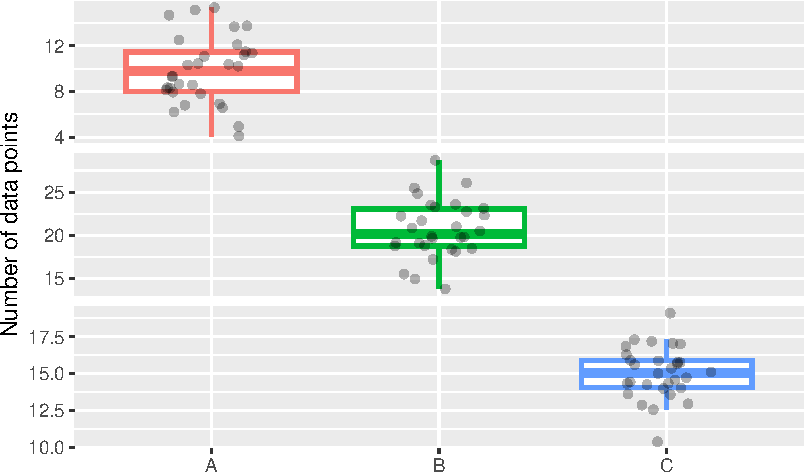
\includegraphics[keepaspectratio]{BCB744_Intro_R_Test_2025_files/figure-pdf/unnamed-chunk-28-1.pdf}}

\subsection{Question 6}\label{question-6-1}

For this assessment, you will analyse the built-in R dataset
\texttt{datasets::UKDriverDeaths}, which contains monthly totals of car
drivers killed or seriously injured in road accidents in Great Britain
from January 1969 to December 1984. This time series data allows for
examination of long-term trends, seasonal patterns, and potential
correlations with societal factors.

\begin{enumerate}
\def\labelenumi{\alph{enumi}.}
\tightlist
\item
  \textbf{Data Exploration and Preparation}

  \begin{enumerate}
  \def\labelenumii{\roman{enumii}.}
  \tightlist
  \item
    Load the \texttt{UKDriverDeaths} dataset and examine its structure.
    Convert the time series data into a standard data frame format with
    separate columns for:

    \begin{itemize}
    \tightlist
    \item
      Year
    \item
      Month (both as a number and as a factor with proper names)
    \item
      Number of deaths/injuries
    \end{itemize}
  \item
    Create a new variable that classifies each month into seasons
    (Winter: Dec-Feb, Spring: Mar-May, Summer: Jun-Aug, Autumn:
    Sep-Nov).
  \item
    Create another variable identifying whether each observation falls
    during a major energy crisis period (e.g., the oil crises of
    1973-1974 and 1979-1980).
  \item
    Identify and handle any potential inconsistencies or issues in the
    dataset that might affect subsequent analyses.
  \end{enumerate}
\end{enumerate}

\textbf{{[}20 marks{]}}

\textbf{Answer}

\begin{Shaded}
\begin{Highlighting}[]
\CommentTok{\# Load the dataset}
\FunctionTok{data}\NormalTok{(}\StringTok{"UKDriverDeaths"}\NormalTok{, }\AttributeTok{package =} \StringTok{"datasets"}\NormalTok{)}

\CommentTok{\# Examine the structure}
\FunctionTok{str}\NormalTok{(UKDriverDeaths)}
\end{Highlighting}
\end{Shaded}

\begin{verbatim}
 Time-Series [1:192] from 1969 to 1985: 1687 1508 1507 1385 1632 ...
\end{verbatim}

\begin{Shaded}
\begin{Highlighting}[]
\CommentTok{\# Convert the time series data into a standard data frame format}
\NormalTok{df }\OtherTok{\textless{}{-}} \FunctionTok{data.frame}\NormalTok{(}
  \AttributeTok{Year =} \FunctionTok{floor}\NormalTok{(}\FunctionTok{time}\NormalTok{(UKDriverDeaths)),}
  \AttributeTok{Month =}\NormalTok{ month.abb[}\FunctionTok{cycle}\NormalTok{(UKDriverDeaths)], }
  \AttributeTok{Deaths =} \FunctionTok{as.numeric}\NormalTok{(UKDriverDeaths)}
\NormalTok{)}

\FunctionTok{head}\NormalTok{(df)}
\end{Highlighting}
\end{Shaded}

\begin{verbatim}
  Year Month Deaths
1 1969   Jan   1687
2 1969   Feb   1508
3 1969   Mar   1507
4 1969   Apr   1385
5 1969   May   1632
6 1969   Jun   1511
\end{verbatim}

\begin{Shaded}
\begin{Highlighting}[]
\CommentTok{\# Create a new variable for seasons}
\NormalTok{df }\OtherTok{\textless{}{-}}\NormalTok{ df }\SpecialCharTok{|\textgreater{}}
  \FunctionTok{mutate}\NormalTok{(}\AttributeTok{Season =} \FunctionTok{case\_when}\NormalTok{(}
\NormalTok{    Month }\SpecialCharTok{\%in\%} \FunctionTok{c}\NormalTok{(}\StringTok{"Dec"}\NormalTok{, }\StringTok{"Jan"}\NormalTok{, }\StringTok{"Feb"}\NormalTok{) }\SpecialCharTok{\textasciitilde{}} \StringTok{"Winter"}\NormalTok{,}
\NormalTok{    Month }\SpecialCharTok{\%in\%} \FunctionTok{c}\NormalTok{(}\StringTok{"Mar"}\NormalTok{, }\StringTok{"Apr"}\NormalTok{, }\StringTok{"May"}\NormalTok{) }\SpecialCharTok{\textasciitilde{}} \StringTok{"Spring"}\NormalTok{,}
\NormalTok{    Month }\SpecialCharTok{\%in\%} \FunctionTok{c}\NormalTok{(}\StringTok{"Jun"}\NormalTok{, }\StringTok{"Jul"}\NormalTok{, }\StringTok{"Aug"}\NormalTok{) }\SpecialCharTok{\textasciitilde{}} \StringTok{"Summer"}\NormalTok{,}
\NormalTok{    Month }\SpecialCharTok{\%in\%} \FunctionTok{c}\NormalTok{(}\StringTok{"Sep"}\NormalTok{, }\StringTok{"Oct"}\NormalTok{, }\StringTok{"Nov"}\NormalTok{) }\SpecialCharTok{\textasciitilde{}} \StringTok{"Autumn"}
\NormalTok{  ))}

\CommentTok{\# Create a variable for major energy crisis periods}
\NormalTok{df }\OtherTok{\textless{}{-}}\NormalTok{ df }\SpecialCharTok{|\textgreater{}}
  \FunctionTok{mutate}\NormalTok{(}\AttributeTok{Energy\_Crisis =} \FunctionTok{case\_when}\NormalTok{(}
\NormalTok{    Year }\SpecialCharTok{\%in\%} \DecValTok{1973}\SpecialCharTok{:}\DecValTok{1974} \SpecialCharTok{|}\NormalTok{ Year }\SpecialCharTok{\%in\%} \DecValTok{1979}\SpecialCharTok{:}\DecValTok{1980} \SpecialCharTok{\textasciitilde{}} \StringTok{"Yes"}\NormalTok{,}
    \ConstantTok{TRUE} \SpecialCharTok{\textasciitilde{}} \StringTok{"No"}
\NormalTok{  ))}

\CommentTok{\# Check for inconsistencies}
\FunctionTok{head}\NormalTok{(df)}
\end{Highlighting}
\end{Shaded}

\begin{verbatim}
  Year Month Deaths Season Energy_Crisis
1 1969   Jan   1687 Winter            No
2 1969   Feb   1508 Winter            No
3 1969   Mar   1507 Spring            No
4 1969   Apr   1385 Spring            No
5 1969   May   1632 Spring            No
6 1969   Jun   1511 Summer            No
\end{verbatim}

\begin{Shaded}
\begin{Highlighting}[]
\FunctionTok{tail}\NormalTok{(df)}
\end{Highlighting}
\end{Shaded}

\begin{verbatim}
    Year Month Deaths Season Energy_Crisis
187 1984   Jul   1222 Summer            No
188 1984   Aug   1284 Summer            No
189 1984   Sep   1444 Autumn            No
190 1984   Oct   1575 Autumn            No
191 1984   Nov   1737 Autumn            No
192 1984   Dec   1763 Winter            No
\end{verbatim}

\begin{Shaded}
\begin{Highlighting}[]
\FunctionTok{summary}\NormalTok{(df)}
\end{Highlighting}
\end{Shaded}

\begin{verbatim}
      Year         Month               Deaths        Season         
 Min.   :1969   Length:192         Min.   :1057   Length:192        
 1st Qu.:1973   Class :character   1st Qu.:1462   Class :character  
 Median :1976   Mode  :character   Median :1631   Mode  :character  
 Mean   :1976                      Mean   :1670                     
 3rd Qu.:1980                      3rd Qu.:1851                     
 Max.   :1984                      Max.   :2654                     
 Energy_Crisis     
 Length:192        
 Class :character  
 Mode  :character  
                   
                   
                   
\end{verbatim}

\begin{enumerate}
\def\labelenumi{\alph{enumi}.}
\setcounter{enumi}{1}
\tightlist
\item
  \textbf{Temporal Trend Analysis}

  \begin{enumerate}
  \def\labelenumii{\roman{enumii}.}
  \tightlist
  \item
    Create a comprehensive visualisation showing the full time series
    with:

    \begin{itemize}
    \tightlist
    \item
      Clear temporal trends
    \item
      A smoothed trend line
    \item
      Vertical lines or shading indicating major UK policy changes
      related to road safety (e.g., 1983 seat belt law)
    \item
      Annotations for key events
    \end{itemize}
  \item
    Develop a visualisation examining monthly fatality averages across
    the entire period, ordered appropriately to show seasonal patterns.
  \item
    Create a visualisation that compares annual patterns between the
    first half of the dataset (1969-1976) and the second half
    (1977-1984).
  \item
    Using \emph{tidy} data manipulation techniques, calculate and
    visualise the year-over-year percent change in fatalities for each
    month throughout the dataset.
  \end{enumerate}
\end{enumerate}

\textbf{{[}20 marks{]}}

\textbf{Answer}

\begin{Shaded}
\begin{Highlighting}[]
\CommentTok{\# i. Full time series visualisation}
\FunctionTok{ggplot}\NormalTok{(df, }\FunctionTok{aes}\NormalTok{(}\AttributeTok{x =} \FunctionTok{as.Date}\NormalTok{(}\FunctionTok{paste}\NormalTok{(Year, Month, }\StringTok{"01"}\NormalTok{, }\AttributeTok{sep =} \StringTok{"{-}"}\NormalTok{),}
                           \AttributeTok{format =} \StringTok{"\%Y{-}\%b{-}\%d"}\NormalTok{), }\AttributeTok{y =}\NormalTok{ Deaths)) }\SpecialCharTok{+}
  \FunctionTok{geom\_line}\NormalTok{() }\SpecialCharTok{+}
  \FunctionTok{geom\_smooth}\NormalTok{(}\AttributeTok{method =} \StringTok{"loess"}\NormalTok{, }\AttributeTok{se =} \ConstantTok{FALSE}\NormalTok{, }\AttributeTok{color =} \StringTok{"red"}\NormalTok{) }\SpecialCharTok{+}
  \FunctionTok{geom\_vline}\NormalTok{(}\AttributeTok{xintercept =} \FunctionTok{as.Date}\NormalTok{(}\FunctionTok{c}\NormalTok{(}\StringTok{"1983{-}01{-}01"}\NormalTok{)), }\AttributeTok{linetype =} \StringTok{"dashed"}\NormalTok{) }\SpecialCharTok{+}
  \FunctionTok{annotate}\NormalTok{(}\StringTok{"text"}\NormalTok{, }\AttributeTok{x =} \FunctionTok{as.Date}\NormalTok{(}\StringTok{"1983{-}01{-}01"}\NormalTok{), }\AttributeTok{y =} \DecValTok{200}\NormalTok{, }\AttributeTok{label =} \StringTok{"Seat belt law"}\NormalTok{, }\AttributeTok{vjust =} \SpecialCharTok{{-}}\DecValTok{1}\NormalTok{) }\SpecialCharTok{+}
  \FunctionTok{labs}\NormalTok{(}\AttributeTok{x =} \StringTok{"Year"}\NormalTok{, }\AttributeTok{y =} \StringTok{"Deaths"}\NormalTok{, }\AttributeTok{title =} \StringTok{"UK Driver Deaths 1969{-}1984"}\NormalTok{) }\SpecialCharTok{+}
  \FunctionTok{theme\_minimal}\NormalTok{()}
\end{Highlighting}
\end{Shaded}

\pandocbounded{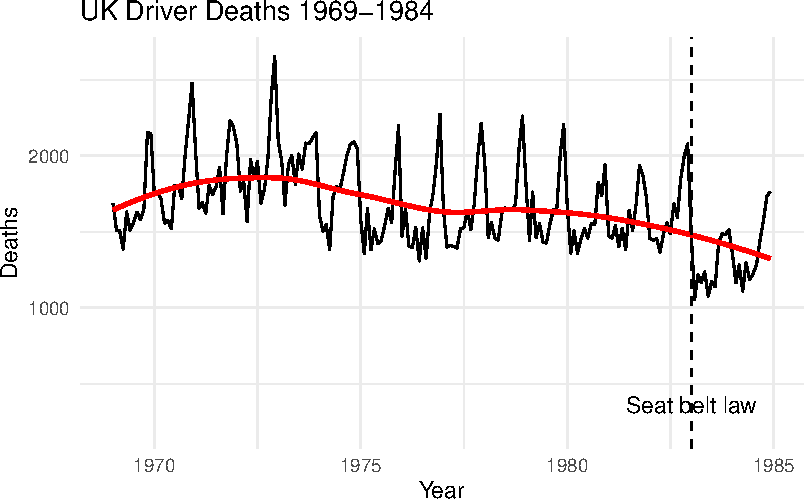
\includegraphics[keepaspectratio]{BCB744_Intro_R_Test_2025_files/figure-pdf/unnamed-chunk-30-1.pdf}}

\begin{Shaded}
\begin{Highlighting}[]
\CommentTok{\# ii. Monthly fatality averages}
\CommentTok{\# ensure the months are ordered correctly and include also}
\CommentTok{\# SD for each month (as determined across the years)}
\NormalTok{df}\SpecialCharTok{$}\NormalTok{Month }\OtherTok{\textless{}{-}} \FunctionTok{factor}\NormalTok{(df}\SpecialCharTok{$}\NormalTok{Month, }\AttributeTok{levels =}\NormalTok{ month.abb)}

\FunctionTok{ggplot}\NormalTok{(df, }\FunctionTok{aes}\NormalTok{(}\AttributeTok{x =}\NormalTok{ Month, }\AttributeTok{y =}\NormalTok{ Deaths, }\AttributeTok{fill =}\NormalTok{ Season)) }\SpecialCharTok{+}
  \FunctionTok{geom\_bar}\NormalTok{(}\AttributeTok{stat =} \StringTok{"summary"}\NormalTok{, }\AttributeTok{fun =} \StringTok{"mean"}\NormalTok{, }\AttributeTok{position =} \StringTok{"dodge"}\NormalTok{) }\SpecialCharTok{+}
  \FunctionTok{geom\_errorbar}\NormalTok{(}\AttributeTok{stat =} \StringTok{"summary"}\NormalTok{, }\AttributeTok{fun.data =} \StringTok{"mean\_se"}\NormalTok{, }\AttributeTok{position =} \StringTok{"dodge"}\NormalTok{) }\SpecialCharTok{+}
  \FunctionTok{labs}\NormalTok{(}\AttributeTok{x =} \StringTok{"Month"}\NormalTok{, }\AttributeTok{y =} \StringTok{"Average Deaths"}\NormalTok{, }\AttributeTok{fill =} \StringTok{"Season"}\NormalTok{) }\SpecialCharTok{+}
  \FunctionTok{theme\_minimal}\NormalTok{()}
\end{Highlighting}
\end{Shaded}

\pandocbounded{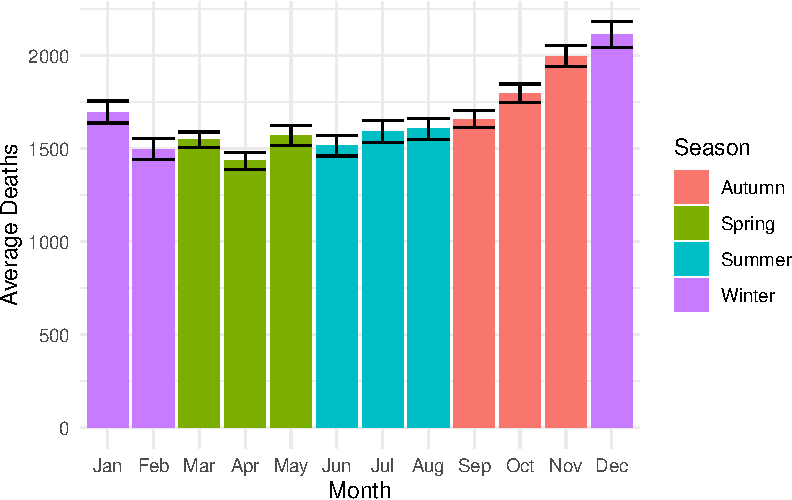
\includegraphics[keepaspectratio]{BCB744_Intro_R_Test_2025_files/figure-pdf/unnamed-chunk-31-1.pdf}}

\begin{Shaded}
\begin{Highlighting}[]
\CommentTok{\# iii. Annual patterns comparison}
\CommentTok{\# ensure the years are ordered correctly and that the SDs are presented}
\NormalTok{df }\OtherTok{\textless{}{-}}\NormalTok{ df }\SpecialCharTok{|\textgreater{}}
  \FunctionTok{mutate}\NormalTok{(}\AttributeTok{Half =} \FunctionTok{case\_when}\NormalTok{(}
\NormalTok{    Year }\SpecialCharTok{\%in\%} \DecValTok{1969}\SpecialCharTok{:}\DecValTok{1976} \SpecialCharTok{\textasciitilde{}} \StringTok{"First Half"}\NormalTok{,}
\NormalTok{    Year }\SpecialCharTok{\%in\%} \DecValTok{1977}\SpecialCharTok{:}\DecValTok{1984} \SpecialCharTok{\textasciitilde{}} \StringTok{"Second Half"}
\NormalTok{  ))}

\FunctionTok{ggplot}\NormalTok{(df, }\FunctionTok{aes}\NormalTok{(}\AttributeTok{x =}\NormalTok{ Month, }\AttributeTok{y =}\NormalTok{ Deaths, }\AttributeTok{fill =}\NormalTok{ Half)) }\SpecialCharTok{+}
  \FunctionTok{geom\_bar}\NormalTok{(}\AttributeTok{stat =} \StringTok{"summary"}\NormalTok{, }\AttributeTok{fun =} \StringTok{"mean"}\NormalTok{, }\AttributeTok{position =} \StringTok{"dodge"}\NormalTok{) }\SpecialCharTok{+}
  \FunctionTok{geom\_errorbar}\NormalTok{(}\AttributeTok{stat =} \StringTok{"summary"}\NormalTok{, }\AttributeTok{fun.data =} \StringTok{"mean\_se"}\NormalTok{, }\AttributeTok{position =} \StringTok{"dodge"}\NormalTok{) }\SpecialCharTok{+}
  \FunctionTok{labs}\NormalTok{(}\AttributeTok{x =} \StringTok{"Month"}\NormalTok{, }\AttributeTok{y =} \StringTok{"Average Deaths"}\NormalTok{, }\AttributeTok{fill =} \StringTok{"Period"}\NormalTok{) }\SpecialCharTok{+}
  \FunctionTok{theme\_minimal}\NormalTok{()}
\end{Highlighting}
\end{Shaded}

\pandocbounded{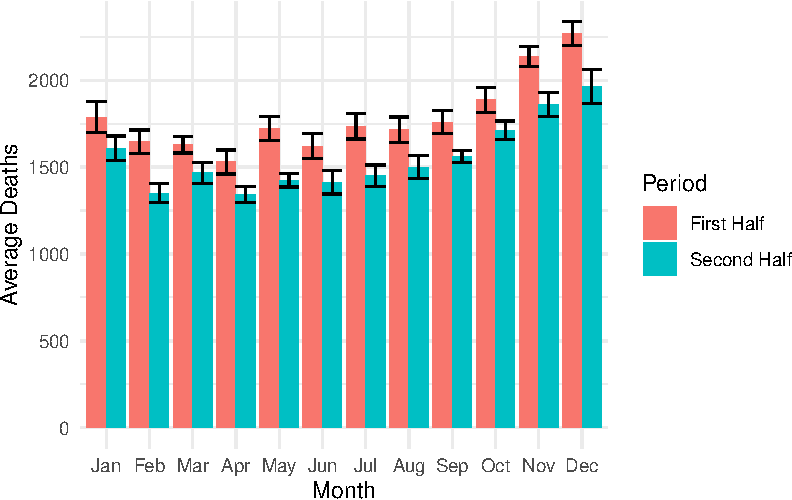
\includegraphics[keepaspectratio]{BCB744_Intro_R_Test_2025_files/figure-pdf/unnamed-chunk-32-1.pdf}}

\begin{Shaded}
\begin{Highlighting}[]
\CommentTok{\# iv. Year{-}over{-}year percent change}
\NormalTok{df\_yoy }\OtherTok{\textless{}{-}}\NormalTok{ df }\SpecialCharTok{\%\textgreater{}\%}
  \FunctionTok{arrange}\NormalTok{(Year, Month) }\SpecialCharTok{\%\textgreater{}\%}           \CommentTok{\# ensure rows are in ascending time order}
  \FunctionTok{group\_by}\NormalTok{(Month) }\SpecialCharTok{\%\textgreater{}\%}               \CommentTok{\# group so that we compare same months}
  \FunctionTok{mutate}\NormalTok{(}\AttributeTok{Deaths\_Pct\_Change =}        \CommentTok{\# (current {-} previous) / previous * 100}
    \DecValTok{100} \SpecialCharTok{*}\NormalTok{ (Deaths }\SpecialCharTok{{-}} \FunctionTok{lag}\NormalTok{(Deaths)) }\SpecialCharTok{/} \FunctionTok{lag}\NormalTok{(Deaths)}
\NormalTok{  ) }\SpecialCharTok{\%\textgreater{}\%}
  \FunctionTok{ungroup}\NormalTok{()}

\CommentTok{\# Plot year{-}over{-}year \% changes in a facetted bar chart}
\FunctionTok{ggplot}\NormalTok{(df\_yoy, }\FunctionTok{aes}\NormalTok{(}\AttributeTok{x =}\NormalTok{ Year, }\AttributeTok{y =}\NormalTok{ Deaths\_Pct\_Change)) }\SpecialCharTok{+}
  \FunctionTok{geom\_col}\NormalTok{(}\AttributeTok{fill =} \StringTok{"steelblue"}\NormalTok{) }\SpecialCharTok{+}
  \FunctionTok{facet\_wrap}\NormalTok{(}\SpecialCharTok{\textasciitilde{}}\NormalTok{ Month, }\AttributeTok{nrow =} \DecValTok{3}\NormalTok{) }\SpecialCharTok{+}
  \FunctionTok{labs}\NormalTok{(}
    \AttributeTok{x =} \StringTok{"Year"}\NormalTok{,}
    \AttributeTok{y =} \StringTok{"Year{-}over{-}year \% change in Deaths"}
\NormalTok{  ) }\SpecialCharTok{+}
  \FunctionTok{theme}\NormalTok{(}
    \AttributeTok{axis.text.x =} \FunctionTok{element\_text}\NormalTok{(}\AttributeTok{angle =} \DecValTok{90}\NormalTok{, }\AttributeTok{vjust =} \FloatTok{0.5}\NormalTok{)}
\NormalTok{  ) }\SpecialCharTok{+}
  \FunctionTok{scale\_x\_discrete}\NormalTok{(}
    \AttributeTok{breaks =} \FunctionTok{c}\NormalTok{(}\StringTok{"1969"}\NormalTok{, }\StringTok{"1974"}\NormalTok{, }\StringTok{"1979"}\NormalTok{, }\StringTok{"1984"}\NormalTok{)  }\CommentTok{\# Adjust as you wish}
\NormalTok{  )}
\end{Highlighting}
\end{Shaded}

\pandocbounded{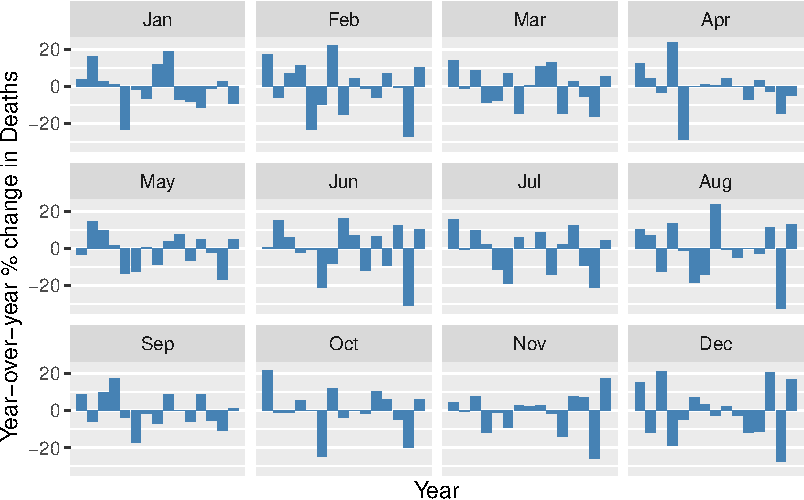
\includegraphics[keepaspectratio]{BCB744_Intro_R_Test_2025_files/figure-pdf/unnamed-chunk-33-1.pdf}}

\begin{enumerate}
\def\labelenumi{\alph{enumi}.}
\setcounter{enumi}{2}
\tightlist
\item
  \textbf{Pattern Analysis and Decomposition}

  \begin{enumerate}
  \def\labelenumii{\roman{enumii}.}
  \tightlist
  \item
    Calculate and visualise the average number of fatalities by season
    across all years.
  \item
    Create a heatmap showing fatalities by month and year, with
    appropriate color scaling to highlight temporal clusters.
  \item
    Implement a decomposition of the time series to separate: - The
    overall trend - Seasonal patterns - Remaining variation
  \item
    Visualise each component and discuss what factors might contribute
    to the patterns observed.
  \end{enumerate}
\end{enumerate}

Note: Some of this will be new to you. But don't worry, use any means
available to you to solve the problem.

\textbf{{[}25 marks{]}}

\textbf{Answer}

\begin{Shaded}
\begin{Highlighting}[]
\CommentTok{\# i. Average fatalities by season: mean with SD}
\NormalTok{df\_season }\OtherTok{\textless{}{-}}\NormalTok{ df }\SpecialCharTok{\%\textgreater{}\%}
  \FunctionTok{group\_by}\NormalTok{(Season) }\SpecialCharTok{\%\textgreater{}\%}
  \FunctionTok{summarise}\NormalTok{(}
    \AttributeTok{Avg\_Deaths =} \FunctionTok{mean}\NormalTok{(Deaths),}
    \AttributeTok{SD\_Deaths  =} \FunctionTok{sd}\NormalTok{(Deaths)}
\NormalTok{  )}

\FunctionTok{ggplot}\NormalTok{(df\_season, }\FunctionTok{aes}\NormalTok{(}\AttributeTok{x =}\NormalTok{ Season, }\AttributeTok{y =}\NormalTok{ Avg\_Deaths)) }\SpecialCharTok{+}
  \FunctionTok{geom\_col}\NormalTok{(}\AttributeTok{fill =} \StringTok{"steelblue"}\NormalTok{) }\SpecialCharTok{+}
  \FunctionTok{geom\_errorbar}\NormalTok{(}
    \FunctionTok{aes}\NormalTok{(}
      \AttributeTok{ymin =}\NormalTok{ Avg\_Deaths }\SpecialCharTok{{-}}\NormalTok{ SD\_Deaths,}
      \AttributeTok{ymax =}\NormalTok{ Avg\_Deaths }\SpecialCharTok{+}\NormalTok{ SD\_Deaths}
\NormalTok{    ),}
    \AttributeTok{width =} \FloatTok{0.2}
\NormalTok{  ) }\SpecialCharTok{+}
  \FunctionTok{labs}\NormalTok{(}
    \AttributeTok{x =} \StringTok{"Season"}\NormalTok{,}
    \AttributeTok{y =} \StringTok{"Average Deaths"}\NormalTok{,}
    \AttributeTok{title =} \StringTok{"Average Deaths by Season"}
\NormalTok{  ) }\SpecialCharTok{+}
  \FunctionTok{theme\_minimal}\NormalTok{()}
\end{Highlighting}
\end{Shaded}

\pandocbounded{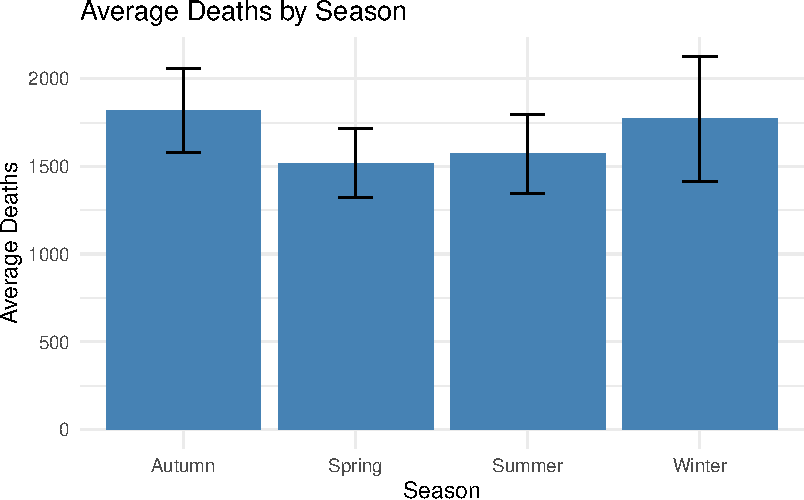
\includegraphics[keepaspectratio]{BCB744_Intro_R_Test_2025_files/figure-pdf/unnamed-chunk-34-1.pdf}}

\begin{Shaded}
\begin{Highlighting}[]
\CommentTok{\# ii. Heatmap of fatalities by month and year}
\FunctionTok{ggplot}\NormalTok{(df, }\FunctionTok{aes}\NormalTok{(}\AttributeTok{x =}\NormalTok{ Month, }\AttributeTok{y =}\NormalTok{ Year, }\AttributeTok{fill =}\NormalTok{ Deaths)) }\SpecialCharTok{+}
  \FunctionTok{geom\_tile}\NormalTok{() }\SpecialCharTok{+}
  \FunctionTok{scale\_fill\_viridis\_c}\NormalTok{() }\SpecialCharTok{+}
  \FunctionTok{labs}\NormalTok{(}\AttributeTok{x =} \StringTok{"Month"}\NormalTok{, }\AttributeTok{y =} \StringTok{"Year"}\NormalTok{, }\AttributeTok{fill =} \StringTok{"Deaths"}\NormalTok{) }\SpecialCharTok{+}
  \FunctionTok{theme\_minimal}\NormalTok{()}
\end{Highlighting}
\end{Shaded}

\pandocbounded{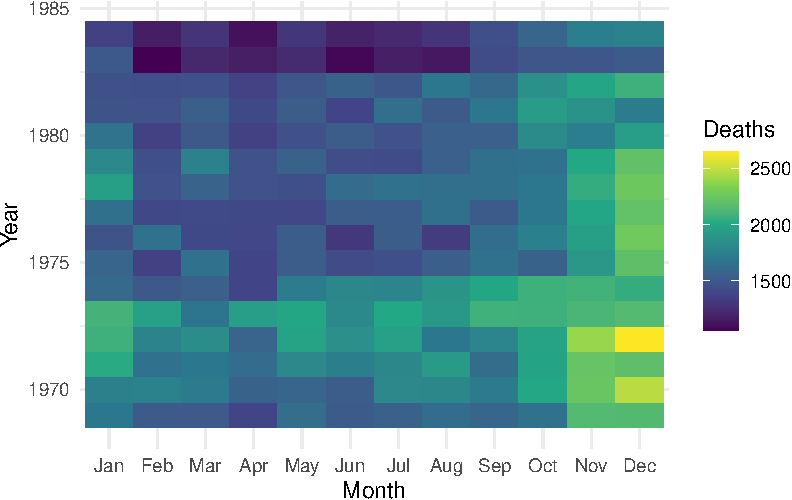
\includegraphics[keepaspectratio]{BCB744_Intro_R_Test_2025_files/figure-pdf/unnamed-chunk-35-1.pdf}}

\begin{Shaded}
\begin{Highlighting}[]
\CommentTok{\# iii. Time series decomposition}
\CommentTok{\# Decompose the time series into trend, seasonal, and remainder components}
\CommentTok{\# First, convert df to a time{-}series (ts) object in chronological order}
\NormalTok{df\_ts }\OtherTok{\textless{}{-}}\NormalTok{ df }\SpecialCharTok{\%\textgreater{}\%}
  \FunctionTok{arrange}\NormalTok{(Year, Month) }\SpecialCharTok{\%\textgreater{}\%}
  \FunctionTok{pull}\NormalTok{(Deaths) }\SpecialCharTok{\%\textgreater{}\%}
  \FunctionTok{ts}\NormalTok{(}\AttributeTok{start =} \FunctionTok{c}\NormalTok{(}\DecValTok{1969}\NormalTok{, }\DecValTok{1}\NormalTok{), }\AttributeTok{frequency =} \DecValTok{12}\NormalTok{)  }

\CommentTok{\# Then, decompose using classical decomposition}
\NormalTok{ts\_decomposed }\OtherTok{\textless{}{-}} \FunctionTok{decompose}\NormalTok{(df\_ts, }\AttributeTok{type =} \StringTok{"additive"}\NormalTok{)}

\CommentTok{\# iv. Plot the results}
\FunctionTok{plot}\NormalTok{(ts\_decomposed)}
\end{Highlighting}
\end{Shaded}

\pandocbounded{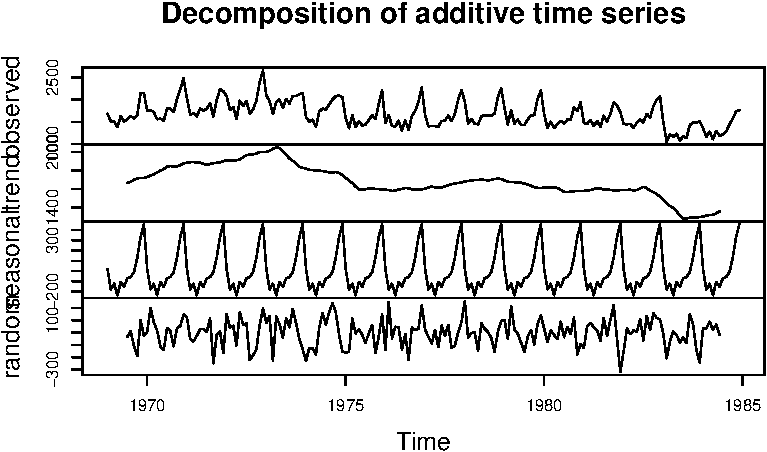
\includegraphics[keepaspectratio]{BCB744_Intro_R_Test_2025_files/figure-pdf/unnamed-chunk-36-1.pdf}}

\begin{enumerate}
\def\labelenumi{\alph{enumi}.}
\setcounter{enumi}{3}
\tightlist
\item
  \textbf{Data manipulation}
\end{enumerate}

Starting with the data as presented in the \texttt{UKDriverDeaths}
dataset, create a new dataframe identical to the \texttt{Seatbelts}
dataset.

\textbf{{[}5 marks{]}}

\textbf{Answer}

The two datasets differ substantially in structure and content.
\texttt{Seatbelts} has columns for drivers, front passengers, rear
passengers, \# (etc.), while \texttt{UKDriverDeaths} only has a
measurement variable for the total number of drivers regardless of
whether or not they were killed or where in the vehicle they were,
etc\ldots{} So, we cannot perfectly recreate the \texttt{Seatbelts}
dataset from the \texttt{UKDriverDeaths} dataset. However, we can create
a column with the total drivers only\ldots{}

\begin{Shaded}
\begin{Highlighting}[]
\CommentTok{\# Look at the original \textasciigrave{}Seatbelts\textasciigrave{} dataset}
\FunctionTok{data}\NormalTok{(}\StringTok{"Seatbelts"}\NormalTok{, }\AttributeTok{package =} \StringTok{"datasets"}\NormalTok{)}
\FunctionTok{head}\NormalTok{(Seatbelts)}
\end{Highlighting}
\end{Shaded}

\begin{verbatim}
     DriversKilled drivers front rear   kms PetrolPrice VanKilled law
[1,]           107    1687   867  269  9059   0.1029718        12   0
[2,]            97    1508   825  265  7685   0.1023630         6   0
[3,]           102    1507   806  319  9963   0.1020625        12   0
[4,]            87    1385   814  407 10955   0.1008733         8   0
[5,]           119    1632   991  454 11823   0.1010197        10   0
[6,]           106    1511   945  427 12391   0.1005812        13   0
\end{verbatim}

\begin{Shaded}
\begin{Highlighting}[]
\FunctionTok{data}\NormalTok{(}\StringTok{"UKDriverDeaths"}\NormalTok{, }\AttributeTok{package =} \StringTok{"datasets"}\NormalTok{)}
\NormalTok{UKDriverDeaths}
\end{Highlighting}
\end{Shaded}

\begin{verbatim}
      Jan  Feb  Mar  Apr  May  Jun  Jul  Aug  Sep  Oct  Nov  Dec
1969 1687 1508 1507 1385 1632 1511 1559 1630 1579 1653 2152 2148
1970 1752 1765 1717 1558 1575 1520 1805 1800 1719 2008 2242 2478
1971 2030 1655 1693 1623 1805 1746 1795 1926 1619 1992 2233 2192
1972 2080 1768 1835 1569 1976 1853 1965 1689 1778 1976 2397 2654
1973 2097 1963 1677 1941 2003 1813 2012 1912 2084 2080 2118 2150
1974 1608 1503 1548 1382 1731 1798 1779 1887 2004 2077 2092 2051
1975 1577 1356 1652 1382 1519 1421 1442 1543 1656 1561 1905 2199
1976 1473 1655 1407 1395 1530 1309 1526 1327 1627 1748 1958 2274
1977 1648 1401 1411 1403 1394 1520 1528 1643 1515 1685 2000 2215
1978 1956 1462 1563 1459 1446 1622 1657 1638 1643 1683 2050 2262
1979 1813 1445 1762 1461 1556 1431 1427 1554 1645 1653 2016 2207
1980 1665 1361 1506 1360 1453 1522 1460 1552 1548 1827 1737 1941
1981 1474 1458 1542 1404 1522 1385 1641 1510 1681 1938 1868 1726
1982 1456 1445 1456 1365 1487 1558 1488 1684 1594 1850 1998 2079
1983 1494 1057 1218 1168 1236 1076 1174 1139 1427 1487 1483 1513
1984 1357 1165 1282 1110 1297 1185 1222 1284 1444 1575 1737 1763
\end{verbatim}

\begin{Shaded}
\begin{Highlighting}[]
\CommentTok{\# Create a new dataframe identical to the Seatbelts dataset}
\NormalTok{Seatbelts\_v2 }\OtherTok{\textless{}{-}} \FunctionTok{data.frame}\NormalTok{(}
  \AttributeTok{drivers =}\NormalTok{ UKDriverDeaths}
\NormalTok{)}
\FunctionTok{head}\NormalTok{(Seatbelts\_v2)}
\end{Highlighting}
\end{Shaded}

\begin{verbatim}
  drivers
1    1687
2    1508
3    1507
4    1385
5    1632
6    1511
\end{verbatim}

\textbf{TOTAL MARKS: 160}

\textbf{-- THE END --}




\end{document}
